%%%%%%%%%%%%%%%%%%%% author.tex %%%%%%%%%%%%%%%%%%%%%%%%%%%%%%%%%%%
%
% sample root file for your "contribution" to a contributed volume
%
% Use this file as a template for your own input.
%
%%%%%%%%%%%%%%%% Springer %%%%%%%%%%%%%%%%%%%%%%%%%%%%%%%%%%


% RECOMMENDED %%%%%%%%%%%%%%%%%%%%%%%%%%%%%%%%%%%%%%%%%%%%%%%%%%%
\documentclass[graybox]{svmult}

% choose options for [] as required from the list
% in the Reference Guide

\usepackage{mathptmx}       % selects Times Roman as basic font
\usepackage{helvet}         % selects Helvetica as sans-serif font
\usepackage{courier}        % selects Courier as typewriter font
\usepackage{type1cm}        % activate if the above 3 fonts are
                            % not available on your system
%
\usepackage{makeidx}         % allows index generation
\usepackage{graphicx}        % standard LaTeX graphics tool
                             % when including figure files
\usepackage{multicol}        % used for the two-column index
\usepackage[bottom]{footmisc}% places footnotes at page bottom

% see the list of further useful packages
% in the Reference Guide

\makeindex             % used for the subject index
                       % please use the style svind.ist with
                       % your makeindex program

%%%%%%%%%%%%%%%%%%%%%%%%%%%%%%%%%%%%%%%%%%%%%%%%%%%%%%%%%%%%%%%%%%%%%%%%%%%%%%%%%%%%%%%%%

%%%%%%%%%%%%%%%%%%%%%%  Our packages and macros   %%%%%%%%%%%%%%%%%%%%%%%%%%%%%%%%%%%%%%%

% numbers option provides compact numerical references in the text. 
\usepackage[numbers]{natbib}
%\usepackage{multicol}
\usepackage[bookmarks=true]{hyperref}
\usepackage{color}
%\usepackage{graphicx}
%\usepackage{subfloat}
\usepackage{textcomp}
%\usepackage{amsthm}
%\usepackage{amsfonts}
\usepackage{subcaption}
\usepackage{algorithm}
\usepackage{algpseudocode}
\usepackage{pbox}
\usepackage[normalem]{ulem}

%\theoremstyle{definition}
%\newtheorem{definition}{Definition}[section]
\usepackage{amsmath}

\renewcommand{\algorithmicrequire}{\textbf{Input:}}
\renewcommand{\algorithmicensure}{\textbf{Output:}}

%% Tarik's Shortcuts
% For marking TODOs in an obvious way
\newcommand{\TODO}[1]{ {\bf \textcolor{red}{TODO:} #1 }}
\newcommand{\abj}[1]{\textcolor{blue}{#1}}
\newcommand{\dbj}[1]{\textcolor{blue}{\sout{#1}}}
\newcommand{\cbj}[2]{\textcolor{blue}{\sout{#1}}\textcolor{blue}{~#2}}
\newcommand{\abt}[1]{\textcolor{magenta}{#1}}
\usepackage{amsbsy}
\usepackage{overpic}


%%%%%%%%%%%%%%%%%%%%%%%%%%%%%%%%%%%%%%%%%%%%%%%%%%%%%%%%%%%%%%%%%%%%%%%%%%%%%%%%%%%%%%%%%



\begin{document}

\title*{Computer-Aided Compositional Design and Verification for Modular Robots}

% You will get a Paper-ID when submitting a pdf file to the conference system
\author{Tarik Tosun$^*$, Gangyuan Jing$^*$, Hadas Kress-Gazit, and Mark Yim}

\institute{
Tarik Tosun \at University of Pennsylvania, Philadelphia PA, \email{tarikt@grasp.upenn.edu}
\and Gangyuan Jing \at Cornell University, Ithaca NY, \email{gj56@cornell.edu}
\and Hadas Kress-Gazit \at Cornell University, Ithaca NY, \email{hadaskg@cornell.edu}
\and Mark Yim \at University of Pennsylvania, Philadelphia PA, \email{yim@grasp.upenn.edu}
\and $^*$ Tarik Tosun and Gangyuan Jing contributed equally to this work.
}

\maketitle

\abstract{To take full advantage of the flexibility of a modular robot system,
users must be able to create new configurations and behaviors quickly. We
present a design framework  that facilitates  rapid creation of new
configurations and behaviors through composition of existing ones, and tools to
verify configurations and behaviors as they are being created. New
configurations are created by combining existing sub-configurations, for example
combining four legs and a body to create a walking robot. Behaviors are
associated with each configuration, so that when sub-configurations are
composed, their associated behaviors are immediately available for composition
as well. We introduce a new motion description language (Series-Parallel Action
Graphs) that facilitates the rapid creation of complex behaviors by composition
of simpler behaviors. We provide tools that automatically verify configurations
and behaviors during the design process, allowing the user to identify problems
early and iterate quickly. After verification, users can  evaluate their
configurations and behaviors in a physical simulator. The software we have
developed is open-source, and will be made freely available online.}

\section{Introduction} 

Modular reconfigurable robot systems have been studied extensively for several
decades.  These systems distinguish themselves from conventional robotic systems in their ability to transform into different shapes to address a wide variety of tasks. They promise to be versatile, robust, and low cost
\cite{yim2000polybot}. Dozens of groups have different kinds of reconfigurable robots\cite{fukuda1990cellular, lipson2000towards}, and introduced approaches for
programming them \cite{salemi2001hormone, stoy2002using,
zhang2003phase}.  Over 800 papers, a book \cite{stoy2010book}, and a survey \cite{yim2007modular} have been written on the subject.

This versatility places an additional burden on the user, because
solving problems with modular robots involves not only designing  programs,
but also the best physical form for the task at hand. If this
complexity is not appropriately managed, it will present a significant barrier to
using modular robots to address practical tasks \cite{yim2000modular}. If the user is free to create any new design to
solve a new task, but must program the design from scratch every time, creating
new designs will be a huge amount of effort, and the advantage of versatile modular
hardware will be defeated.

Software modularity is a well-established practice for developing large
maintainable systems and avoiding duplication of effort. In robotics, software
behaviors are inextricably linked to the hardware they control, resulting in challenges to making modularity effective. Strong
ties to physical hardware also increase the need for software verification, to ensure
that hardware is not damaged. Significant progress has been made on these fronts
in traditional robotics, most notably
ROS \cite{Quigley2009} which provides inter-process communication and standard libraries for common robot tasks,
as well as powerful verification tools \cite{huang2014rosrv}.
  
In modular robotics, the challenge is different.  Modular robot systems are not optimized
for specific tasks, so in order for them to be useful, we must take full advantage of their flexibility. To do
so, a user must be able to generate and verify configurations and behaviors
as quickly as possible.  

Toward that end, we present a design framework that facilitates the rapid creation
of new configurations
and behaviors through composition, and tools to verify configurations and behaviors
while they are being created. New configurations are created by combining existing
sub-configurations,
for example combining four legs and a body to create a walking robot.
Behaviors are associated with each configuration, so that when sub-configurations
are composed, their associated behaviors are immediately available for composition
as well.
We introduce a new motion description language (Series-Parallel Action Graphs)
that facilitates the rapid creation of complex behaviors by composition of simpler
behaviors.
We provide tools that automatically verify configurations and behaviors during the
design process, allowing the user to identify problems early and iterate quickly.
After verification, users can  evaluate their configurations and behaviors in a physical simulator.
The software we have developed is open-source, and will be made freely available
online.

The remainder of this paper provides a  description of the
structure and algorithmic components of our framework.  In Section \ref{sec:related-work},
we discuss relevant background material.
In Section \ref{sec:preliminaries} we introduce terminology and  concepts used elsewhere in the
paper. 
In Section \ref{sec:approach}, we describe the algorithmic basis
for the three major components of our framework - design composition, behavior
composition, and verification.  In Section
\ref{sec:implementation}, we discuss the open-source software
tools used to implement our framework. In Section \ref{sec:examples}, we provide examples highlighting
important aspects of the framework, including a demonstration of the user's
workflow.  We demonstrate that our framework saves the
user time and effort, and allows him or her to easily develop complex and
capable designs.

\section{Related Work} \label{sec:related-work} 
In some respects, our work parallels the efforts of Mehta \cite{mehta2014design}
and Bezzo \cite{bezzo2014demo}, who aim to create and program printable robots
from novice users' design specifications.  Users create new designs by composing
existing elements from a design library, and appropriate circuitry and control
software are automatically generated as physical designs are assembled. The
framework we present is intended specifically for modular robots, and
consequently the workflow and design considerations are fundamentally different
from that presented by Mehta and Bezzo.  In traditional robot design (or
printable robot design), hardware and software are somewhat decoupled - hardware
is designed and built once, and then programmed many times.  In the case of a
modular robot system, the system can be reconfigured to meet new tasks, so
hardware configuration and behavior programming go hand in hand.  We intend our
system to be fast enough that the user could conceivably develop and program a
new design for every new task - designs are built once, and programmed once.
Where Mehta et al. provide many facilities to generate and verify low-level
behaviors (\textit{e.g.} motor drivers appropriate for motors), we do so for
high-level behaviors.

A significant amount of work has been done in developing behaviors and software
for modular robots. Much of this work focused on automatically generating
designs and behaviors using artificial intelligence systems. Genetic algorithms
have been applied for the automated generation of designs and behaviors
\cite{hornby2003generative}. Other work has focused on distributed control
\cite{walter2002choosing} and hormone-based control \cite{salemi2001hormone}.

Efforts have also been made to generate behaviors by automatically identifying the ``role'' a module should play based on its place in a connected structure \cite{stoy2002using}.  Functionality is propagated downward: based on a high-level goal (like ``walk'') and a connected structure of modules, functional sub-structures (like legs and a spine) are automatically identified, and modules are directed to execute appropriate roles in a distributed fashion.  In our work, modular structures are similarly associated with appropriate behaviors. Rather than identifying roles in a top-down fashion, we build designs with the desired functionality from the bottom up. The use creates new designs by composing sub-components and associated behaviors from a library, building a new structure that can definitely execute the desired behavior.

While significant progress has been made in the automated generation of modular
robot behaviors, automated systems are not yet capable of making modular robots
truly useful in practice \cite{yim2007modular}.  The need for new programming
techniques to manage the complexity of modular robot systems has been
acknowledged in the literature \cite{yim2000modular}. Historically, gait tables
have been a commonly used format in which open-loop kinematic behaviors can be
easily encoded \cite{yim1994locomotion}. Phased automata have also been
presented as a way to easily create scalable gaits for large numbers of modular
robots \cite{zhang2003phase}. In this paper, we introduce a novel motion
description language that enables users to quickly create behaviors for modular
robots.

A number of robot simulators have been developed, including simulators specifically for modular robots \cite{christensen2008unified}. For our work, we opted to use Gazebo \cite{koenig2004design} because of its growing popularity in the robotics community. While our software currently only supports the SMORES robot \cite{Davey2012}, other modular robot designs can easily be incorporated given appropriate SDF files. Future work includes incorporating native support for the ckBot robot \cite{davey2012modlock}.

Our framework assists users in verifying design validity by identifying self-
collision and loss of gravitational stability. In existing literature, these
conditions have been checked in the context of modular robot reconfiguration
planning \cite{casal2001reconfiguration} and motion planning
\cite{yoshida2002self}. To our knowledge, there is no modular robot design tool
that verifies these conditions to provide assistance to a human designer.

\section{Definitions}
\label{sec:preliminaries}
In this section, we present concepts and terms which will be used later in the paper.

\begin{definition}[Module] A module is a small robot that can move, respond to commands,
and attach to other modules.  Formally, we define a  module  as
$\mathcal{M}=({^\mathcal{W}}D^{\mathcal{M}}, X, A,K)$.
The rigid body \textit{displacement}, ${^\mathcal{W}}D^{\mathcal{M}}\in SE(3)$ 
gives the position and orientation of the module body frame in the world  frame $\mathcal{W}$.
The \textit{state} of the module, \(X=\lbrack x_1, x_2, \ldots, x_d \rbrack\),
 is a \(d\)-dimensional vector representing the \(d\) degrees of freedom (DoF) of the module.
$A=\{a_1, a_2, ..., a_k\}$ is the set of \textit{attachment points} where the 
module can connect to other modules.
The  module's \textit{forward kinematics function}, \(K: (X, a_i) \rightarrow SE(3) \) 
returns \({^\mathcal{B}}D^{a_{i}}\) (the displacement of attachment point \(a_i\) 
in the body frame) as a function of \(X\).
% , where:
% \begin{itemize}
% \item ${^\mathcal{W}}D^{\mathcal{M}}\in SE(3)$ is the rigid-body \textit{displacement} (position and orientation)
% of the module body frame in the world reference frame $\mathcal{W}$. 
% \item \(X=\lbrace x_1, x_2, \ldots, x_d \rbrace\) is the \textit{state} of the module,
% with each \(x_i\) corresponding to one of the \(d\) degrees of freedom (DoF) of the module.
% \item $A=\{a_1, a_2, ..., a_k\}$ is the set of \textit{attachment points} where the module can connect to other modules.
% \item \(K: (X, a_i) \rightarrow SE(3) \) is the module's \textit{forward kinematics function}, returning \({^\mathcal{B}}D^{a_{i}}\) (the displacement of attachment point \(a_i\) in the body frame) as a function of \(X\)
% \end{itemize}
%
Figure~\ref{fig:graphical-representations} shows a schematic representation of a module with  four attachment points.
\end{definition}
%
% \begin{figure}
% \begin{center}
%         \begin{subfigure}[b]{0.4\columnwidth}
%                 \begin{center}
%                 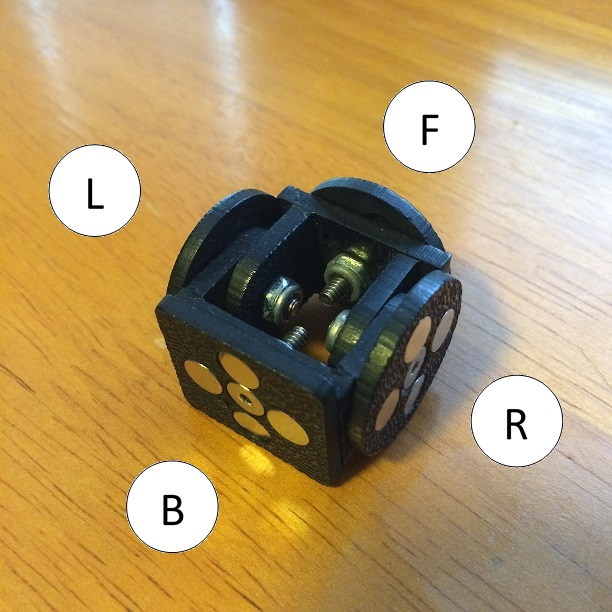
\includegraphics[width=0.7\textwidth]{images/smores.JPG}
%                 \caption{A module}
%                 \end{center}
%                 \label{fig:smores_photo}
%            \end{subfigure}
%            ~
%         \begin{subfigure}[b]{0.4\columnwidth}
%                 \begin{center}
%                 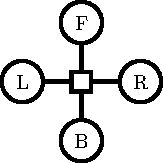
\includegraphics[width=0.7\textwidth]{images/tikz/smores.pdf}
%                 \caption{The graphical representation}
%                 \end{center}
%                 \label{fig:smores_graph}
%         \end{subfigure}
% \end{center}
% \caption{A photo of a module and its graphical representation}
% \label{fig:smores}
% \end{figure}
%
% \begin{figure}
% \sidecaption
% %\begin{center}
%         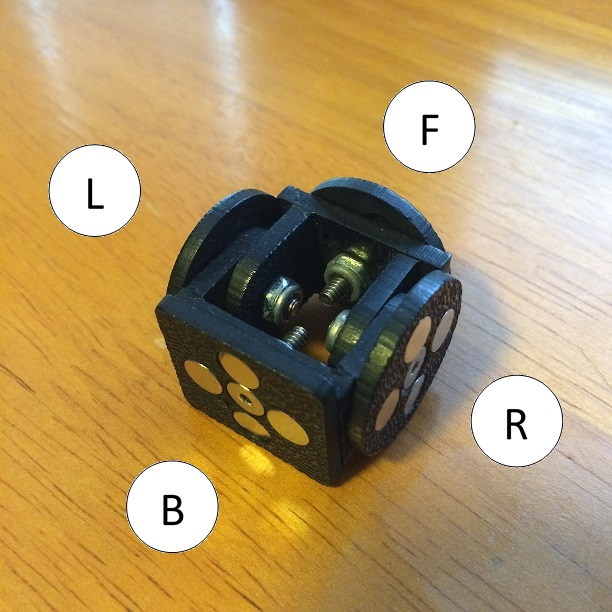
\includegraphics[height=1.1in]{images/smores.JPG}
%         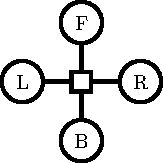
\includegraphics[height=1.1in]{images/tikz/smores.pdf}
% %\end{center}
% \caption{A photo of a module (left) and its graphical representation (right)}
% \label{fig:smores}
% \end{figure}
\begin{figure}
%1 
\begin{overpic}[height=01.0in]{images/smores_robot.png}
  \put(3,30) {(1)}
\end{overpic}
%2 
\begin{overpic}[height=1.0in]{images/tikz/smores.pdf}
  \put(3,8) {(2)}
\end{overpic}
%3
\begin{overpic}[height=1.0in]{images/smores_conf.JPG}
  \put(4,6) {(3)}
\end{overpic}
%4
\begin{overpic}[height=1.0in]{images/tikz/smores_conf.pdf}
  \put(4,6) {(4)}
\end{overpic}
\caption{From left: (1) A photo of a SMORES module with four attachment points
(left, right, front, and back), (2) its graphical representation, (3)
a photo of a configuration with three modules, and (4) its graphical representation.}
\label{fig:graphical-representations}
\end{figure}


\begin{definition}[Configuration]
\label{def:configuration}
A \textit{configuration} is a contiguous set of connected modules which we treat as a
single robot.  The identity of a configuration is determined by its connective structure; configurations
can be represented by graphs with nodes representing modules and edges
representing connections between modules.   Individual modules
are considered interchangeable (as long as they are of the same kind).

In this paper, we present an object-oriented design framework for modular robot
systems, and treat configurations as the fundamental objects. Rather than defining
configurations only by the topology of their component modules, we define them recursively,
as being composed of connected sub-configurations. A single module is considered the
smallest configuration.

Formally, we define a configuration as $\mathcal{C}=(C_, \gamma, M, E, \delta,
X, B)$.
%
Here, $C=\{\mathcal{C}_{1}, \mathcal{C}_{2}, ..., \mathcal{C}_{q}\}$ is a set of sub-configurations.
%
$\gamma: C \rightarrow 2^M$ is a function {mapping} a configuration \( \mathcal{C}_i \in C\) to its set of modules,  \( M=\bigcup_{\mathcal{C}\in C}{\gamma(\mathcal{C})} \).
%
$E$ is a set of connections between modules. Elements of \(E\) are pairs of
attachment points, $(\mathcal{M}_i.a_i, \mathcal{M}_j.a_j)\in E,$ where $\mathcal{M}_{i},\mathcal{M}_j \in M, \mathcal{M}_i \neq \mathcal{M}_j$, and $a_i\in \mathcal{M}_i.A$, $a_j\in \mathcal{M}_j.A$.
%
The orientation of one attachment point relative another is represented by the
labeling function $\delta: E \rightarrow SO(3)$, returning.
%
The \textit{state} of the configuration is \(X = \bigcup_{\mathcal{M}_i \in M} \mathcal{M}_i.X \).
%
Finally, associated with each configuration is a set of \textit{behaviors} \(B\)
(see Definition~\ref{def:behavior}).

% , where:
% \begin{itemize}
% \item $C$ is a set of sub-configurations, $C=\{\mathcal{C}_{1}, \mathcal{C}_{2}, ..., \mathcal{C}_{q}\}$.
% \item $\gamma: C \rightarrow 2^M$ is a function {mapping} a configuration \( \mathcal{C} \in C\) to its set of modules.
% % Note: if we define a single module as the smallest configuration, we don't have
% % to worry about the case when the configuration contains no configurations.
% \item \( M=\bigcup_{\mathcal{C}\in C}{\gamma(\mathcal{C})} \) is the set of modules.
% %\item $M$ is the set of modules. If this configuration contains no other configurations, i.e. $C = \emptyset$, $M$ is just the set of all modules of this configuration. If this configuration is composed by other configurations, i.e. $C=\{\mathcal{C}_{1}, \mathcal{C}_{2}, ..., \mathcal{C}_{q}\}$, we define $M=\bigcup_{\mathcal{C}\in C}{\gamma(\mathcal{C})}$.
% \item $E$ is a set of connections between modules. $(\mathcal{M}_i.a_i, \mathcal{M}_j.a_j)\in E,$ where $\mathcal{M}_{i},\mathcal{M}_j \in M, \mathcal{M}_i \neq \mathcal{M}_j$, and $a_i\in \mathcal{M}_i.A$, $a_j\in \mathcal{M}_j.A$.
% \item $\delta: E \rightarrow SO(3)$ is a labeling function over connections returning
% \({^{\mathcal{M}_i.a_i}}R^{\mathcal{M}_j.a_j}\), the orientation of one attachment point relative the
% other.
% \item \(X = \displaystyle\bigcup_{\mathcal{M}_i \in M} \mathcal{M}_i.X \) is the \textit{state} of the configuration.
% \item \(B\) is a set of \textit{behaviors} (Definition~\ref{def:behavior}) associated with the configuration.
% \end{itemize}

Figure~\ref{fig:graphical-representations} shows a photo of a configuration composed
of three modules, each with four attachment points, and its
graphical representation. Blue zigzag lines represent connections between
modules, and the label of each connection shows the angle offset of that
connection.
%Assuming acyclic configurations, w
We can compute forward kinematics for the entire
configuration by composing displacements module-to-module. Let any module \(\mathcal{M}_f \in M\) have
fixed displacement \({^\mathcal{W}}D^{\mathcal{B}_f}\) in the world frame.
Let \(\mathcal{M}_i: (\mathcal{M}_i.a_i,~\mathcal{M}_f.a_f) \in E \) be connected to \(\mathcal{M}_f\).
 We can find \({^\mathcal{W}}D^{\mathcal{M}_i}\) by composing displacements as follows:
\begin{align*}
{^\mathcal{W}}D^{\mathcal{M}_i} =& [{^\mathcal{W}}D^{\mathcal{M}_f}] [{^{\mathcal{M}_f}}D^{a_f}][
{^{a_f}}D^{a_i}] [{^{\mathcal{M}_i}}D^{a_i}]^T \\
=& [{^\mathcal{W}}D^{\mathcal{M}_f}] [K_f(X_f,a_f)] \begin{bmatrix} \delta(e) & 0
\\ 0 & 1\end{bmatrix} [K_i(X_i,a_i)]^T
\end{align*}

where \(e=(\mathcal{M}_i.a_i,~\mathcal{M}_f.a_f)\). To find the world-frame displacements
of all other modules, we may traverse the connections of the configuration,  repeatedly
composing displacements in the manner above. 
\end{definition}

% \begin{figure}
% \begin{center}
%         \begin{subfigure}[b]{0.4\columnwidth}
%                 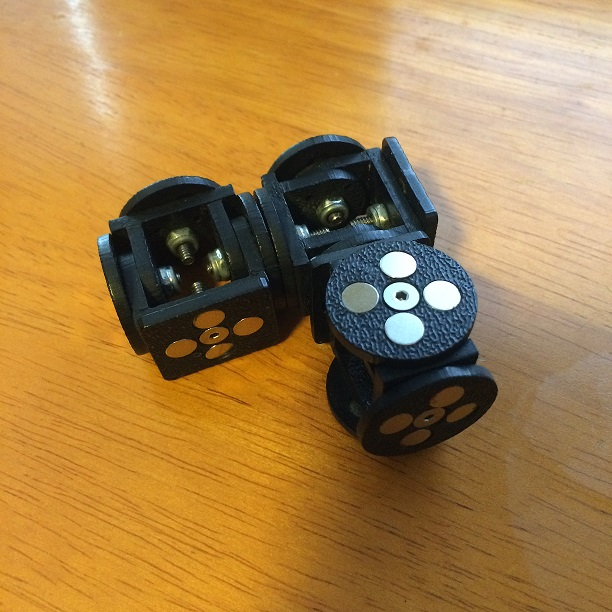
\includegraphics[width=0.7\textwidth]{images/smores_conf.JPG}
%                 \caption{A configuration}
%                 \label{fig:smores_conf_photo}
%         \end{subfigure}
%            ~
%         \begin{subfigure}[b]{0.4\columnwidth}
%                 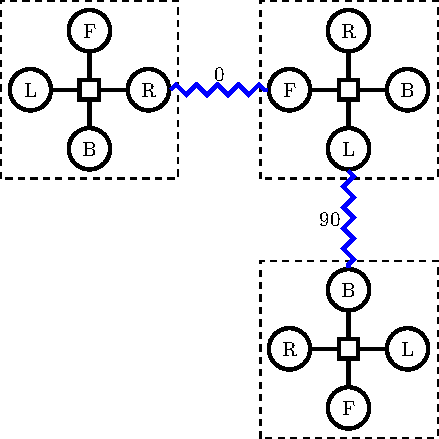
\includegraphics[width=0.7\textwidth]{images/tikz/smores_conf.pdf}
%                 \caption{The graphical representation}
%                 \label{fig:smores_conf_graph}
%         \end{subfigure}
% \end{center}
% \caption{A photo of a configuration with three modules and its graphical representation}
% \label{fig:smores_conf}
% \end{figure}
% \begin{figure}
% \sidecaption
% 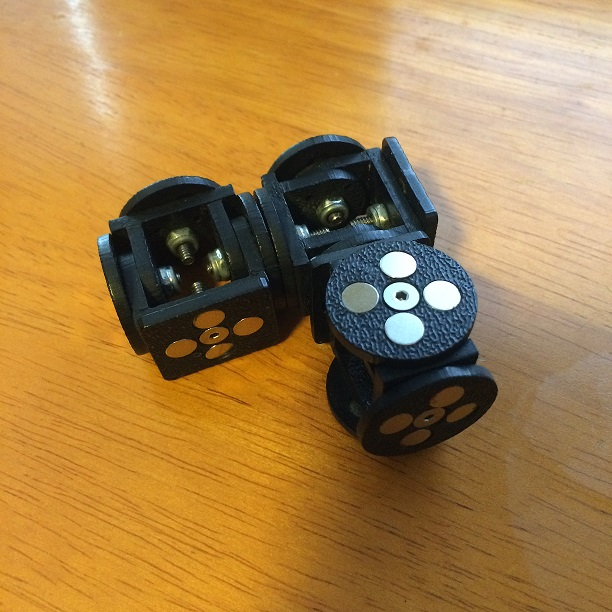
\includegraphics[height=1.2in]{images/smores_conf.JPG}
% 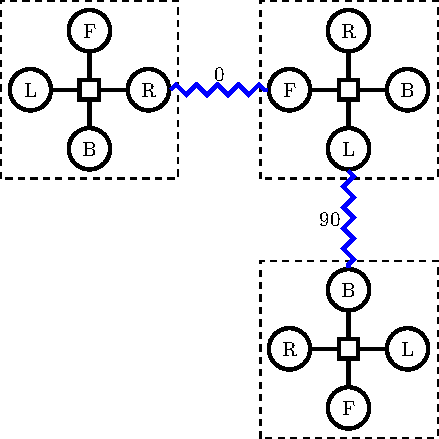
\includegraphics[height=1.2in]{images/tikz/smores_conf.pdf}
% \caption{A photo of a configuration with three modules (left) and its graphical representation (right).}
% \label{fig:smores_conf}
% \end{figure}


\begin{definition}[Behavior]\label{def:behavior}
A \textit{behavior} is a programmed sequence of movements for a specific configuration
intended to produce a desired effect.  A gait for walking is one example.  In
this paper, we consider open-loop kinematic behaviors represented as
series-parallel action graphs, described in detail in section
\ref{sec:behavior-representation}.
\end{definition}
\begin{definition}[Controller]
A \textit{controller} is a position or velocity servo for one DoF of a modular
robot.  A controller takes as input a desired position or angular velocity, and
drives the error between the desired and actual state of the DoF it controls to
zero over time.
\end{definition}

% \begin{definition}[Behavior Conflict]
% When writing a behavior, it is possible to command one controller to
% simultaneously hold more than one desired position; this is known as a
% \textit{behavior conflict}.  Behaviors with conflicts are
% impossible to execute.
% \end{definition}
% \begin{definition}[Self-Collision]
% During execution of a behavior, a \textit{self-collision} can occur when two
% different parts of configuration are commanded to occupy the same location in
% space.  Self-collisions can damage the robot, and are usually unwanted.
% \end{definition}
% \begin{definition}[Gravitational Stability]
% While executing many behaviors, it is desirable to maintain \textit{gravitational
% stability} (also called quasi-static stability).  Informally speaking, a
% robot is gravitationally stable when it is balanced, and gravity does not
% create any net moment on it.  Mathematically, the robot is gravitationally stable
% if the projection of its center of
% mass onto the group plane lies within the convex hull of its load-supporting contact points in the
% ground plane.
% \end{definition}
% \begin{definition}[Maintain Connections and Joint Angles]
% Due to the force limit of mechanisms in each module, there maybe situations, 
% especially during execution of a behavior, when force provided is not sufficient to
% maintain all connections between modules in a configuration, or to maintain all joints at desired positions.
% \end{definition}
% 

\section{Approach and Algorithm} \label{sec:approach} The three major
components of our framework are configuration composition, behavior
composition, and verification of configurations and behaviors.  Together,
these three components provide a streamlined workflow to quickly create
functional robots by leveraging an existing library of designs and behaviors.
Combining existing designs and behaviors into new ones allows users to create
large, complicated, and highly functional designs.

\subsection{Configuration Composition} \label{sec:conf_composition}

Before discussing about configuration composition, we will first define a set of connections $E_C$ between configurations in a given set $C$ as $(\mathcal{C}_i.\mathcal{M}_i.a_i, \mathcal{C}_j.\mathcal{M}_j.a_j) \in E_C$, where $\mathcal{C}_{i},\mathcal{C}_j\in C$, $\mathcal{M}_i \in \gamma(\mathcal{C}_i), \mathcal{M}_j \in \gamma(\mathcal{C}_j)$, and $a_i\in \mathcal{M}_i.A$, $a_j\in \mathcal{M}_j.A$. Similar to the assumption about connections in a configuration, we assume that we form an
acyclic graph with configurations in $C$ as nodes and connections in $E_C$ as edges.
\begin{definition}[Configuration Composition]
Given a set of configurations $C$ and a set $E_C$ of connections between them,
configuration composition combines all configurations in $C$ to a single
configuration $\mathcal{C}^*$ that includes all modules and connections from $C$
and $E_C$. we define the composed configuration to be $\mathcal{C}^*=(C^*, \gamma, M, E, \delta,
X, B)$, where \(C^*\), \(M\), \(E\), and \(B\) are defined as the unions of the
corresponding sets of the sub-configurations in \(C\). The definitions of $\gamma$, \(X\), and $\delta$ remain
unchanged from Definition~\ref{def:configuration}. 
\end{definition}

\subsection{Behavior Composition: Series-Parallel Action Graphs}
\label{sec:behavior-representation}
The modular robotics community has developed a number of languages and  methods
to create behaviors, including gait tables \cite{yim1994locomotion}, phased automata
\cite{zhang2003phase}, hormone-based control \cite{salemi2001hormone},
and role-based control \cite{stoy2002using}. Phased automata, hormone, and role-based
control are typically used to specify a single, cyclic behavior (such as a gait for
locomotion) in a distributed fashion.
These methods have good scaling and robustness properties, but are not well-suited
to specifying  the non-cyclic, globally coordinated behaviors required for many tasks
(like picking up and moving an object with an arm).
  
The simplicity and clarity of gait tables makes them appealing for our
application.  However, gait tables are difficult to re-use, and also hard to
scale to very complicated designs. The  motion description language we present
allows low-level behaviors to be combined in series and parallel to create new
higher-level behaviors, encapsulating complexity and facilitating code re-use.
The resulting programs are precise and expressive, and have a nested structure
that is easy to understand and debug.

%    
% We present a novel motion description language for modular robots.  The
% language aims to balance simplicity and expressiveness, and is designed specifically
% for composition, allowing complex behaviors
% to be rapidly created by combining existing behaviors. 
% Typical motion description languages have atomic elements that represent controller
% commands (set-points and gains) with limited duration \cite{brockett1988computer}.
% Extended motion description languages introduce interrupts to control the duration
% of commands \cite{hristu2003motion}.  Our language distinguishes itself by allowing
% existing behaviors to be easily composed to form new behaviors.

 The atoms of the language are called actions.  Similar to a single entry of a gait
table, an action specifies a controller setpoint for a single DoF of a module.  Unlike
a gait table entry, actions do not have explicit timestamps.  Rather, each action has an associated
interrupt condition, which is a boolean function of the (sensed) state of the robot. Similar
to a state transition in a finite state machine (FSM), when the interrupt condition is met the action is  considered
complete, and  execution moves on to the next actions.  Interrupts allow the programmer
to precisely specify behaviors in a natural way: rather than specifying a timed sequence
of motions, the programmer specifies an ordered sequence of actions and has some
assurance that an action will not begin until the robot has actually achieved the goal
state of the previous action. Actions
may optionally include a timeout, which causes the action to be considered complete
automatically once time runs out.

An important distinction between actions in our language and states in a traditional
FSM is that multiple actions may execute in parallel.   Actions are combined through
parallel and series composition to create behaviors. When two actions are composed in series,
the second begins when the first ends. When composed in parallel they
begin simultaneously, and the following actions do not begin until both complete.
A behavior created using these operations is a directed acyclic graph of actions with
series-parallel structure \cite{valdes1979recognition};  Figure \ref{fig:graph-composition} provides
a visual example. This structure is advantageous because the
 series and parallel composition operations   
remain valid for behaviors of arbitrary size, allowing new behaviors to be easily
created by combining existing behaviors.
 
% The fundamental atoms of the language are called actions.  An \textit{action} is a tuple \(
% (J, X, \xi, T)\), where \(J\) identifies a single DoF of a configuration, \(X\) is a
% controller setpoint for that DoF, \(\xi\) specifies an interrupt
% condition, and T specifies a timeout. When an action executes, the controller
% setpoint (position or velocity) for the specified DoF is changed to the specified
% value. The controller maintains this setpoint until receiving a new one from another
% action. The interrupt condition is a boolean function of the (sensed) state of the DoF \(J\).
% When either the interrupt condition is met or time runs out (whichever comes
% first), the action is considered complete, and the next action  begins. The
% interrupt condition can be set to \(false\) (so that only the timeout has effect),
% and \(T\) can be set to infinity (so that only the interrupt has effect). As an example,
% the action \((~Module0\_L,~ \theta_{set}=\pi,~ \xi:\theta==\pi,~T:\infty~)\) encodes
% ``Command the controller of the left wheel of module zero to maintain a setpoint
% of \(\pi\) radians.  When the encoder of that wheel indicates that \(\pi\) radians
% has actually been reached, consider this action complete and move on.''
%  
% Actions are composed to form behaviors. We define a \textit{behavior} as a directed acyclic graph where nodes are
% actions and edges are transitions between actions.  A behavior \(B\) always has
% two special nodes \(S\) and \(T\), which are the \textit{Start} and
% \textit{   Termination} nodes, respectively.  The smallest behavior consists of
% \(S\), \(T\), and a single action.  Behavior execution follows three simple
% rules:
% 
% \begin{enumerate}
% \item Execution begins at \(S\).  \(S\) completes immediately.
% \item Each action begins execution upon completion of \textit{all} its parent actions.
% \item All sequences of execution end at \(T\).
% \end{enumerate}
% 
% Because execution begins at \(S\) and ends at \(T\), there must be a (directed)
% path from every \(S\) to every node in \(B\), and also from every node in \(B\)
% to \(T\). Since \(B\) is acyclic, it is therefore a \textit{directed series-parallel graph} (SPG).
% SPG's can always be formed recursively by parallel and series composition
% operations \cite{valdes1979recognition}. The parallel composition \(P\) of two behaviors \(B_1\),
% \(B_2\), \(P = Pc(B_1, B_2)\) is the disjoint union of their nodes (actions),
% merging \(S_1\) with \(S_2\) and \(T_1\) with \(T_2\). The series composition
% of \(B_1\), \(B_2\), \(S = Sc(B_1, B_2)\) is created from their disjoint union
% by merging \(T_1\) and \(S_2\), so that \(B_1\) and \(B_2\) execute
% sequentially\footnote{Since the merged node is not an action, we can freely
% omit it and instead draw edges from each of its parent nodes to each of its
% child nodes.}.  Note that if \(B_1\) was itself created through parallel
% composition, \(B_2\) will not begin until all chains of execution of \(B_1\)
% are completed. Figure \ref{fig:graph-composition} provides a visual companion.

\begin{figure}
\begin{center}
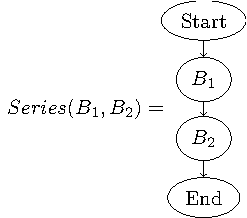
\includegraphics[height=0.8in]{images/tikz/series.pdf}
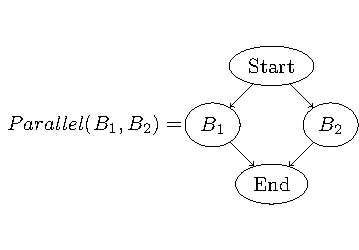
\includegraphics[height=0.8in]{images/tikz/parallel.pdf} \vspace{0.in}
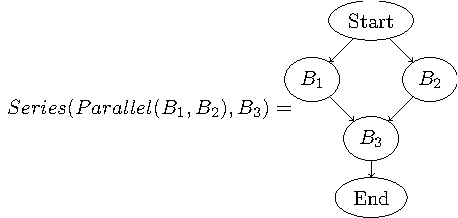
\includegraphics[height=0.8in]{images/tikz/parallel-and-series.pdf}
\end{center}
\caption{Series and parallel composition }
\label{fig:graph-composition}
\end{figure}

%\subsubsection*{Example}
As an example, consider the car design shown in figure \ref{fig:car-and-backhoe}. To create a low-level
``drive-forward'' behavior, we simply command all of its wheels to spin  in parallel.
The car steers by swiveling its central steering column, so a ``turn right''
behavior can be similarly achieved by commanding parallel actions for the steering column joints.
With these low-level behaviors established, we can command trajectories through series
composition, for example: \textit{square=series(drive, turn, drive, turn, drive, turn,
drive, turn)}.

This paradigm  is lightweight enough to code  low-level behaviors quickly and
easily. However, the real value comes from its ability to  combine behaviors
in layers and quickly generate behaviors for complicated designs. This works
particularly well when designs are made by composing smaller designs. For
example, we can easily develop ``drive'' and ``turn''\ behaviors for the
18-module backhoe shown in Figure \ref{fig:car-and-backhoe} by composing  behaviors of
its component car designs: \(driveBackhoe= parallel( driveCar1, driveCar2)\),
and \(turnBackhoe = parallel(turnCar1, turnCar2)\). Each of these one-line
statements commands the movement of  28 degrees of freedom.

We can extend this further to generate a useful high-level behaviors for the
backhoe.  Suppose that the arm has a laser rangefinder attached to the end,
and that we've already created a ``scan'' behavior that sweeps or rotates the
sensor.  We might create a ``patrol'' behavior that scans continuously while
driving in a square: \(patrol = parallel( scan, square)\). Or, if we only want
the robot to scan the corners of a room, we can precisely specify this using
lower-level behaviors:  \(cornerScan=series(drive, scan, turn, drive,scan,
turn, \ldots) \).

Building behaviors in a layered fashion make it much easier
to re-use code.
If primitive behaviors have not yet been built, building a single complicated behavior like ``patrol'' from scratch might  be faster
than first building primitive behaviors and then composing them into the desired
complex behavior. However, the latter process is more efficient in the long run,
because the low-level behaviors can be re-used to quickly create many different
high-level behaviors.

Our emphasis on abstraction begs the question: why not use  a a more fully-featured
plan execution model such as behavior trees \cite{marzinotto2014towards}, or even a
traditional object-oriented programming language (like Java or C++)?  Our
decision was driven by the tradeoff between complexity and ease-of-use: given
our desire for a simplicity and speed of programming, we chose to use an
extremely minimal  paradigm with only two composition operations.
The language is quite expressive: we have used it to develop a number of  complex behaviors
for large designs (see Section \ref{sec:examples}). In the future, we hope to expand
its capabilities without sacrificing ease-of-use.  In particular, facilities
for high-level decision making based on sensed information about the environment
will be a priority.

% \begin{figure}
% \begin{center}
%   \begin{subfigure}[b]{0.4\textwidth}
%     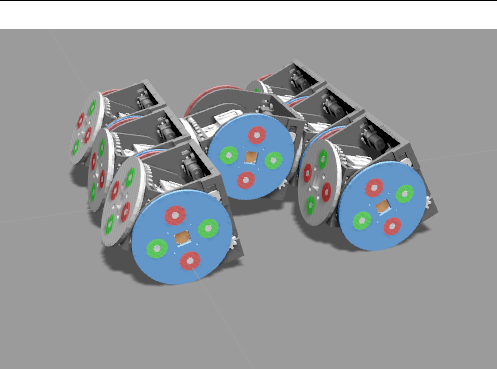
\includegraphics[height=1.1in]{images/library/car.png}
%     \caption{Car design}
%     \label{fig:car-design}
%   \end{subfigure}
%   \begin{subfigure}[b]{0.4\textwidth}
%     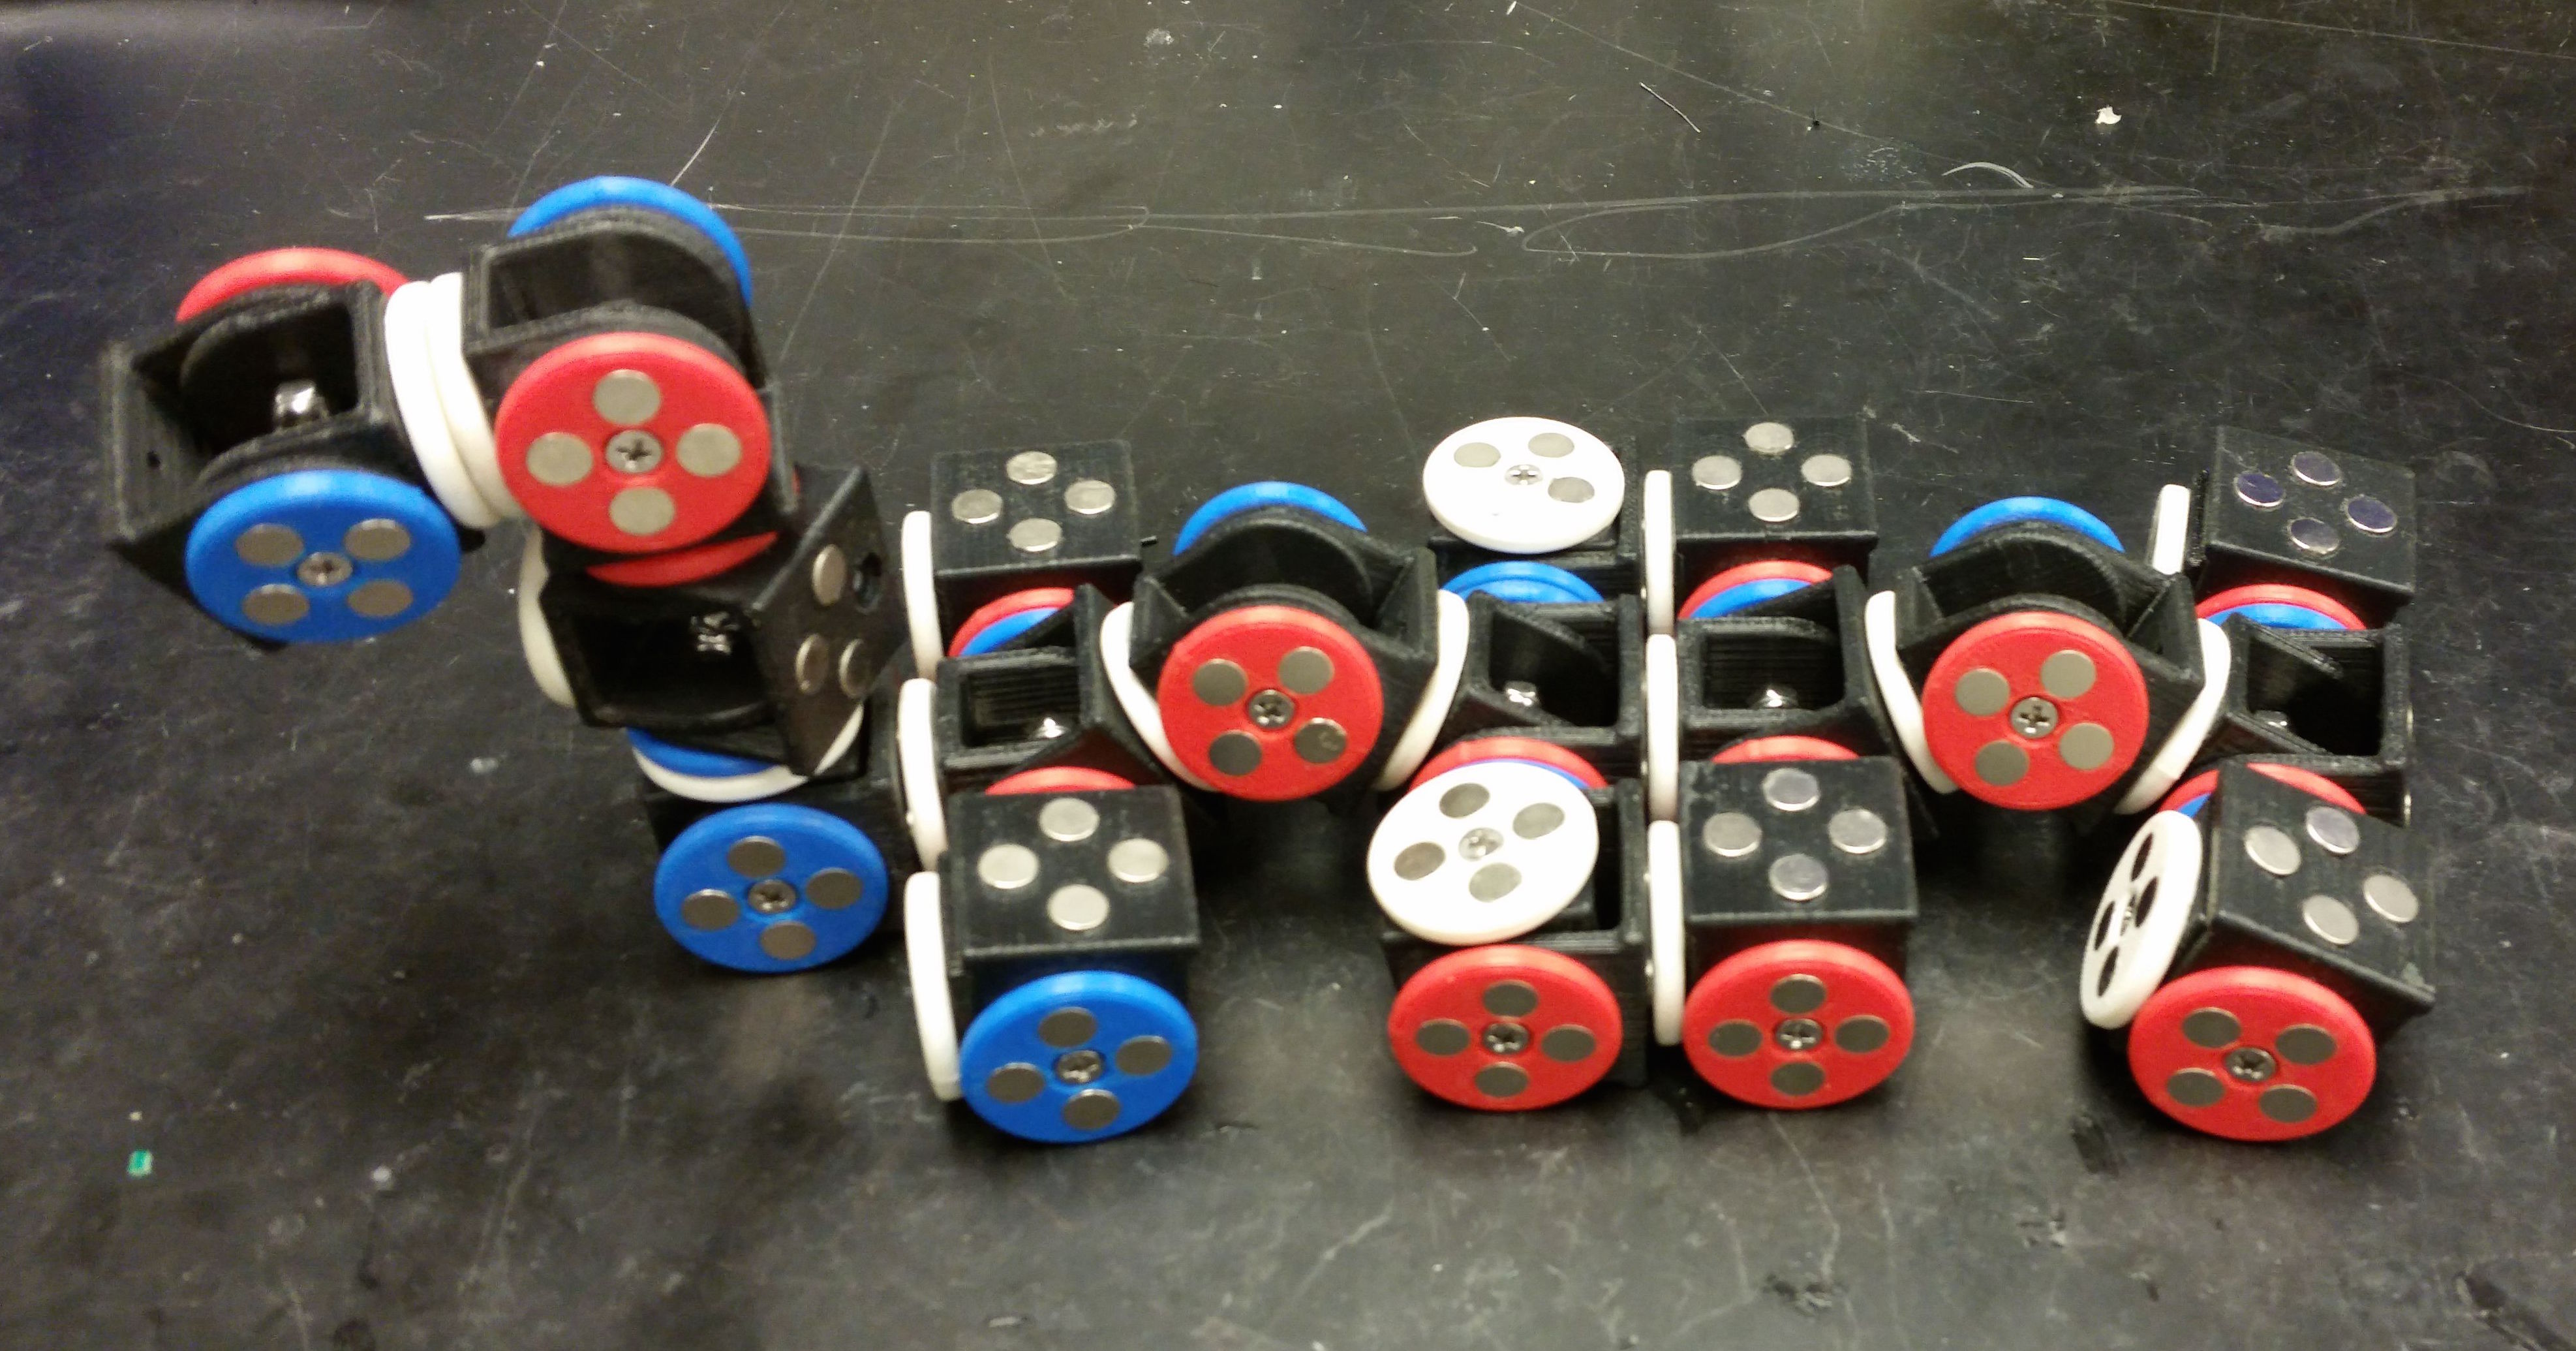
\includegraphics[height=1.1in]{images/library/backhoe.jpeg}
%     \caption{Backhoe design}
%     \label{fig:backhoe-design}
%   \end{subfigure}
% \end{center}
% \end{figure} 
%
\begin{figure}
\begin{center}
    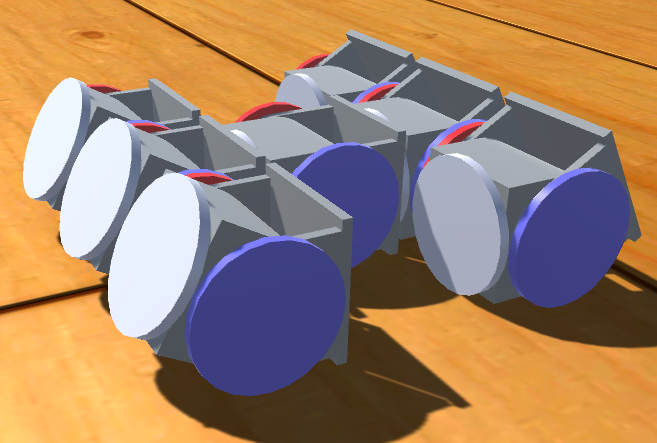
\includegraphics[height=1.1in]{images/library/unity/car.png}
    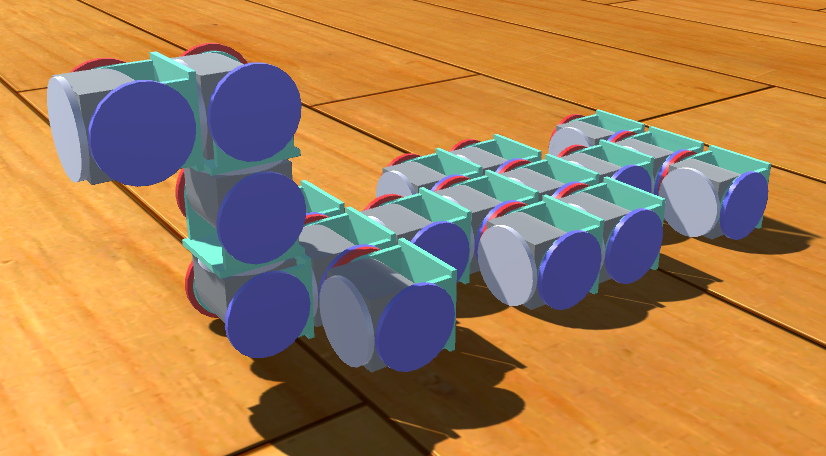
\includegraphics[height=1.1in]{images/library/unity/backhoe.png}
    \caption{Car design (left) and backhoe design (right)}
    \label{fig:car-and-backhoe}
\end{center}
\end{figure} 

% Consider a single module that has two wheels that allow it to drive like a car. To
% drive forward, we might define a DRIVE behavior composing actions for  the left and right wheels
% in parallel:\begin{align*}
% \mathrm{DRIVE} =~~~~~~~~~~~~~~~~~~~~~~~~~~~~~~~~~~~~~~~~~~~~~~~~~~~ \\
% Pc \left( \begin{array}{cccc}
% (~L, & \dot\theta_{set}=6, & \xi:false, & T:5), \\
% (~R, & \dot\theta_{set}=6, & \xi:false, & T:5) \\
% \end{array} \right)\\
% \end{align*}
% The wheels are set to turn at 6 radians per second, and the action will complete
% in 5 seconds.  We might also define a TURN behavior, commanding the wheels to rotate \(\pi\) radians
% in opposite directions:
% \begin{align*}
% \mathrm{TURN} =~~~~~~~~~~~~~~~~~~~~~~~~~~~~~~~~~~~~~~~~~~~~~~~~~~~~~~~~~~~~ \\
% Pc \left( \begin{array}{cccc}
% (~L, & \theta_{set}=\theta_0+\pi, & \xi:\theta==\theta_0+\pi, & T:\infty), \\
% (~R, & \theta_{set}=\theta_0-\pi, & \xi:\theta==\theta_0-\pi, & T:\infty) \\
% \end{array} \right)\\
% \end{align*}
% 
% Here, \(\theta_0\) denotes the currently-sensed value of $\theta$ at the beginning of
% the TURN behavior.
% The action completes when both wheels actually reach their commanded angles of \(\theta_0\pm\pi\). To drive in a square, we compose DRIVE and TURN behaviors in series:
% 
% \begin{align*}
% \mathrm{SQUARE} = Sc (~\mathrm{DRIVE},~\mathrm{TURN},~\mathrm{DRIVE},~\mathrm{TURN},\\
% ~\mathrm{DRIVE},~\mathrm{TURN},~\mathrm{DRIVE},~\mathrm{TURN} )
% \end{align*}
\subsection{ Verification of Configurations and Behaviors} \label{sec:verify}

%\subsubsection{Verification of Configurations \TODO{Consider removing these subsection headings to save space}}\label{sec:verify_conf}
{\bf Verification of Configurations: }
In Section~\ref{sec:conf_composition}, we introduced the definition of configuration composition. During the design process, a user might attempt to compose configurations in a way that is unsafe or physically impossible. We provide facilities to automatically verify designs during construction, saving time that would otherwise be spent simulating or testing invalid designs.

Given a configuration $\mathcal{C}$ and state \(X_0\), we consider to be  $\mathcal{C}$ valid in state \(X_0\) if it is gravitationally stable and free from self
collision between modules.  A robot is gravitationally
stable when it is balanced, and gravity does not create any net moment on it.
If this condition is not met, the robot could tip over and suffer damage.
%
%Mathematically, the robot is \textit{gravitationally stable} if the projection
%of its center of mass onto the group plane lies within the convex hull of its
%load-supporting contact points in the ground plane.
A \textit{self-collision}
occurs when two different parts of configuration are commanded to occupy the
same location in space.  Self-collisions can also cause damage, and are almost
always unwanted.

% However, it might not be
% possible or safe to form the structure represented by the composed configuration
% with the actual modules. Consider the configuration shown in
% Figure~\ref{fig:smores_conf_collision}. It is easy to tell that such
% configuration is not ideal for any task, because the self-collision may damage
% those modules and result in instability of the system. Thus it is important to
% verify whether the configuration is valid or not for a given modular robot
% system.

% \begin{figure}
% \sidecaption
% 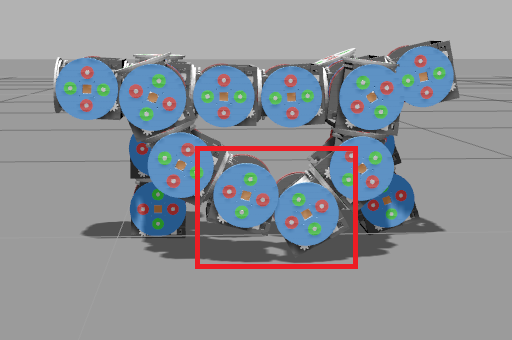
\includegraphics[height=1in]{images/walkbot_collision.png}
% \caption{A configuration with self-collision \TODO{We might consider taking
% this figure out to save space. I think self-collision is easy enough to understand without a picture}}
% \label{fig:smores_conf_collision}
% \end{figure}

% \begin{definition}[Configuration Verification]
% Given a configuration $\mathcal{C}$ and state \(X_0\), we say $\mathcal{C}$ is valid in
% state \(X_0\) if it is gravitationally stable and free from self collision between
% modules.  
% % it satisfied the following set of properties:
% % \begin{itemize}
% % \item There is no collision between modules in the configuration.
% % \item The configuration is gravitationally stable.
% % \end{itemize}
% %Notice that in order to verify the validity of the configuration, one needs to know some properties of all modules for the given modular robot system, e.g. the geometry information, and the mass of each module.
% \end{definition}

We will now describe the methods used to identify gravitational instability and
self-collision. We assume that geometric, kinematic, and mass
information for each module are available. 
%
To check for self-collision, the positions and orientation of all modules are
obtained  through forward kinematics.
%Using the known module geometry, we  check
%whether any two modules occupy the same space. If so, there exists a self-
%collision in the configuration.
Our implementation checks self-collision by
approximating modules as spheres, and checking the distance (radius) between all
pairs. More sophisticated techniques are available which efficiently produce
exact results \cite{pan2012fcl}.
%
Gravitational stability is checked by computing the location of the center of
mass of the configuration based on the known kinematics and mass properties of 
the modules.
% For the given configuration $\mathcal{C}$
% and state \(X_0\), the position of the center of mass is:
% \begin{equation*}
%  P_{\mathcal{C}}=\dfrac{\sum\limits_{\mathcal{M}\in \gamma(\mathcal{C})}{P(\mathcal{M})\cdot \mathcal{M}_m}}{\sum\limits_{\mathcal{M}\in \gamma(\mathcal{C})}{\mathcal{M}_m}}
% \end{equation*}
% where $\mathcal{M}_m$ is the mass of the module $\mathcal{M}$, and
% \(P(\mathcal{M})\) is a function returning the position coordinates of
% \(\mathcal{M}\) in the world frame.
%
We find the set of modules that have minimal position in the $z$ direction and consider them to
be in contact with the ground plane, treating their centroids as an approximate
set of ground contact points.
%A set of points in the $x$-$y$ plane can be extracted from $M_c$ as $\sigma=\{(\mathcal{M}.P.x, \mathcal{M}.P.y)\mid \mathcal{M} \in M_c\}$.
If the projection of the configuration center of mass onto the ground plane
lies within the convex hull of the ground contact points, gravity exerts no
moment and the configuration
is considered statically stable in state \(X_0\).

%\subsubsection{Verification of Behaviors}
\noindent{\bf Verification of Behaviors: }
In Section~\ref{sec:behavior-representation}, we introduced a novel motion description language for modular robots. Like
configurations, behaviors are automatically verified as the user builds them.
  In addition to being free from self-collision and gravitationally stable during
execution, a valid behavior also must not exceed the actuator or connector force
limits of the modules, and must be free from \textit{behavior conflict}.
Since our motion description language allows behaviors to be composed in parallel,
it is possible to compose two behaviors that simultaneously command one controller
to hold more than one desired position; we refer to this as \textit{behavior
conflict}.

  % Actions defined by the language can be combined to produce more complex behaviors. Similar to configuration composition, we want to make sure the composed behaviors are valid and safe to execute. For example, a behavior that results in two modules colliding during the execution should be considered unsafe.
% 
% \begin{definition}[Behavior Verification]
% A behavior is valid if: there are no collisions or behavior conflicts at any time
% during execution, and forces required to maintain all module connections and joint positions do not exceed their limit.
% Additionally, the maximum duration for which the configuration is not
% gravitationally stable during execution is less than a time bound $t_{max}$, and the configuration must be stable at the end of execution.
% \end{definition}

% \begin{definition}[Behavior Verification]
% A behavior is valid if it satisfies the following set of properties when controlling a configuration of a given modular robot system
% \begin{itemize}
% \item Modules do not collide at any time during the execution of the behavior.
% \item There are no behavior conflicts at any time during the execution.
% \item The configuration is gravitationally stable at the end of the execution.
% \item The maximum duration for which the configuration is not gravitationally stable during the execution is less than a time bound $t_{max}$.
% \end{itemize}
% \end{definition}
% State is the right term, so I deleted the TODO.
To verify a behavior with time duration  $T_B$, we discretize execution with sampling time $t_B$. At each time step, we first detect behavior conflict by checking if different commands are given to the same joint of a module simultaneously. If there is no behavior conflict, we update the positions and orientations of all modules in the configuration based on the commands. We then check for self-collision and gravitational instability, using the methods described in section~\ref{sec:verify}.  
A behavior that results in self-collision during a single time step is considered
invalid. For gravitational stability, we specify a time bound
\(t_{max} > t_B\). A behavior is considered unstable if it
includes any period of instability longer than \(t_{max}\), or if the behavior is unstable at time \(T_B\) (at the end).


For checking force limit, we create the model for a module and specify its joint and connection mechanisms in PhysX \cite{PhysX} physics engine with a graphical designing tool called Unity3D \cite{Unity}. By setting the maximum force allowed for the connection between modules and for controlling each joint in the module, we are able to identify a unsafe behavior if we detect, during the behavior execution, any undesired module disconnection or any joint's mismatch between its target position and steady state position
\TODO{Since this is not the implementation section, it might be better to describe
the joint and actuator limit checks without mentioning specific physics engines.
 The specific engines can be included in the implementation section.}.

%\TODO{I have copied this text here from the verification examples section. 
%I think putting it here makes sense, because it helps motivate why we are doing
%behavior verification.  It will also save space, since there is one less section
%heading.  If possible, try to cut down the text as well to save space.}
The need for verification becomes more important as design complexity increases. Consider a four-legged Walkbot example. If the user sets two of the connections with different angle offset, the composed Walkbot configuration will have two legs pointing in the opposite direction of the other two legs, as shown in Figure~\ref{fig:verification}-1. Since the projection of the configuration's center of mass now falls out of the supporting base, the program will warn the user that the configuration is not gravitationally stable. As shown in Figure~\ref{fig:verification}-2, in simulation the configuration quickly fell to the ground due to the instability as warned by the program. 

Verification of behavior design can also aid the user to create valid and safe robot behaviors. When designing the walking behavior for the Walkbot, if the user commands the front and rear leg at the same side of the robot to swing toward each other at the same time, the program will warn the user that there will be collision between some modules in this behavior, as shown in Figure~\ref{fig:verification}-3. The photo shown in Figure~\ref{fig:verification}-4 demonstrates the moment of collision during simulation.

Despite the design of the modular robot system, modules all have limits on maximum force that is available to maintain connections with other modules and to drive each joint to desired positions. Thus, it is crucial to notify the user if there is no sufficient force from module's hardware to execute a behavior while maintaining all modules connections. 
As shown in Figure~\ref{fig:verification}-5, the program detected an undesired disconnection when the user tried to lift a long cantilever arm. Figure~\ref{fig:verification}-6 demonstrates the disconnection in simulation.
 
%\begin{figure}
%\begin{center}
%        \begin{subfigure}[b]{0.48\columnwidth}
%                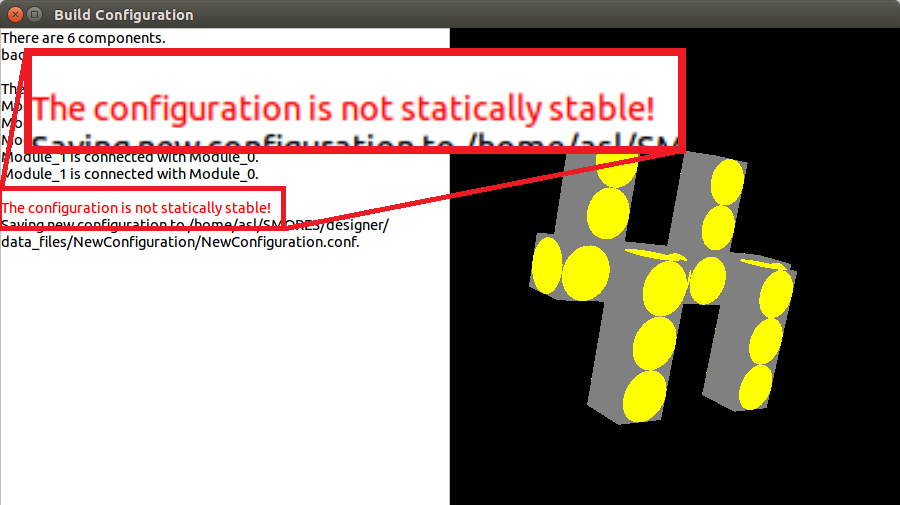
\includegraphics[width=\textwidth]{images/designer_unstable.png}
%                \caption{}
%                \label{fig:designer_unstable}
%           \end{subfigure}
%        \begin{subfigure}[b]{0.48\columnwidth}
%                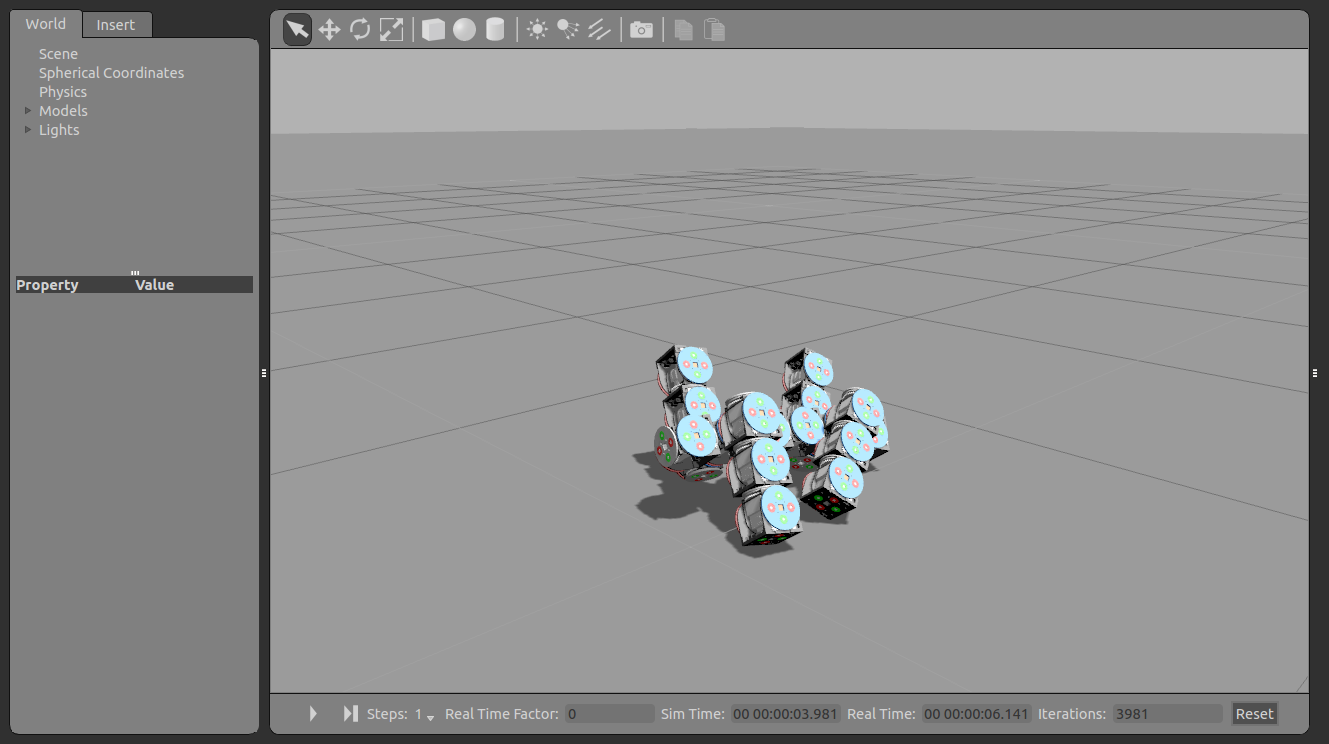
\includegraphics[width=\textwidth]{images/gazebo_unstable2.png}
%                \caption{}
%                \label{fig:gazebo_unstable2}
%        \end{subfigure}
%\end{center}
%\caption{(a) The program warns the composed configuration is not gravitationally stable; (b) The robot fell to ground plane due to instability in simulation}
%\label{fig:unstable}
%\end{figure}
%
%\begin{figure}
%\begin{center}
%        \begin{subfigure}[b]{0.48\columnwidth}
%                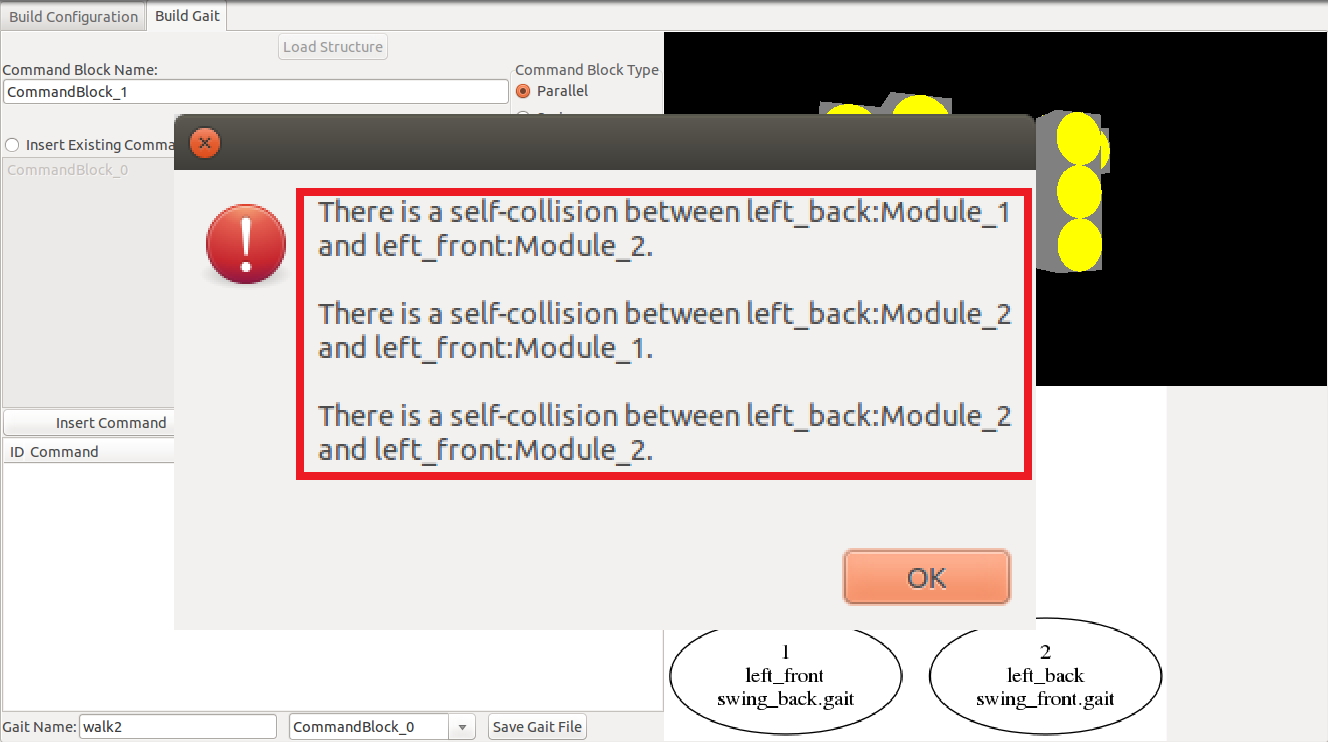
\includegraphics[width=\textwidth]{images/designer_gait_collision.png}
%                \caption{}
%                \label{fig:gait_collision}
%           \end{subfigure}
%        \begin{subfigure}[b]{0.48\columnwidth}
%                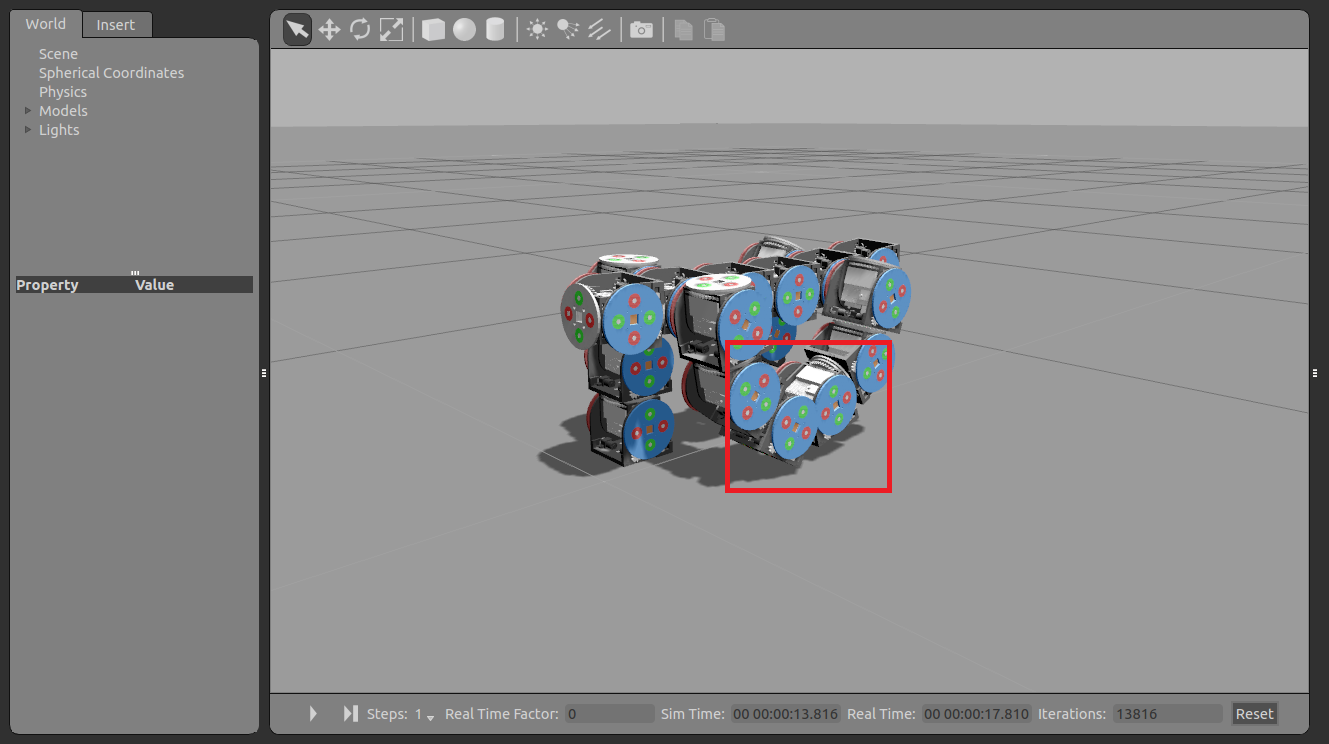
\includegraphics[width=\textwidth]{images/gazebo_gait_collision.png}
%                \caption{}
%                \label{fig:gait_collision2}
%        \end{subfigure}
%\end{center}
%\caption{(a) The program indicates there is collision during the behavior execution; (b) Two feet of  the robot collided during simulation}
%\label{fig:gait_unstable}
%\end{figure}
%
%\begin{figure}
%\begin{center}
%        \begin{subfigure}[b]{0.48\columnwidth}
%                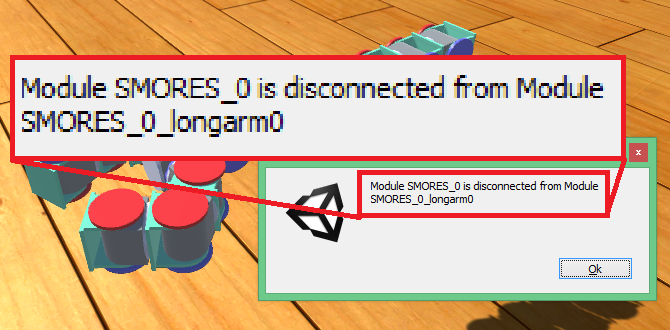
\includegraphics[width=\textwidth]{images/library/unity/breakJoint.png}
%                \caption{}
%                \label{fig:break_joint1}
%           \end{subfigure}
%        \begin{subfigure}[b]{0.48\columnwidth}
%                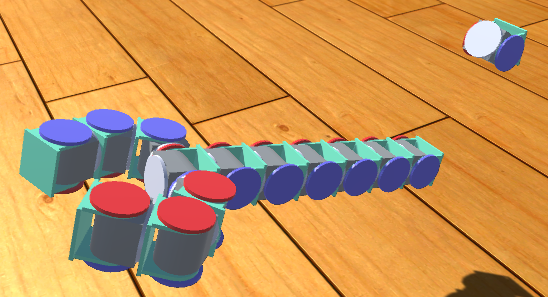
\includegraphics[width=\textwidth]{images/library/unity/breakJoint2.png}
%                \caption{}
%                \label{fig:break_joint2}
%        \end{subfigure}
%\end{center}
%\caption{(a) The program indicates there is undesired disconnection; (b) The configuration disconnected during simulation}
%\label{fig:break_joint}
%\end{figure}

\begin{figure}
%1 
\begin{overpic}[width=0.5\textwidth]{images/gazebo_unstable.png}
  \put(4,6) {(1)}
\end{overpic}
%2 
\begin{overpic}[width=0.5\textwidth]{images/gazebo_unstable2.png}
  \put(4,6) {(2)}
\end{overpic}
%3
\begin{overpic}[width=0.5\textwidth]{images/designer_gait_collision.png}
  \put(4,6) {(3)}
\end{overpic}
%4
\begin{overpic}[width=0.5\textwidth]{images/gazebo_gait_collision.png}
  \put(4,6) {(4)}
\end{overpic}
%5
\begin{overpic}[width=0.5\textwidth]{images/library/unity/breakJoint.png}
  \put(4,6) {(5)}
\end{overpic}
%6
\begin{overpic}[width=0.5\textwidth]{images/library/unity/breakJoint2.png}
  \put(4,6) {(6)}
\end{overpic}
\caption{From top and left: (1) The program warns the composed configuration is not gravitationally stable; (2) The robot fell to ground plane due to instability in simulation; (3)
The program indicates there is collision during the behavior execution; (4) Two feet of  the robot collided during simulation; (5) The program indicates there is undesired disconnection; (6) The configuration disconnected during simulation.}
\label{fig:verification}
\end{figure}

%\subsection{Complexity}
%\TODO{Discuss the complexity of the algorithm with respect to the number of modules and size of gait tables.}

\section{Implementation }
\label{sec:implementation}
Our implementation currently supports only the SMORES modular robot \cite{Davey2012},  but
could easily  incorporate any other modular robot for which an SDF description is available
\TODO{is this true? And should we cite SDF?}. Each SMORES modules has four DoF
- three continuously rotating faces called {\em turntables} and one
central hinge with a 180\textdegree\ range of motion (Figure~\ref{fig:graphical-representations}-1). The
DoF marked 1, 2, and 4 have rotational axes that are parallel and coincident.
Each SMORES module can drive around as a two-wheel differential
drive robot.
SMORES modules may connect to one another via magnets on each of their four
faces, and are capable of  self-reconfiguration.
Formally, we denote the state of a SMORES module as \(X=\lbrace \theta_L, \theta_R,
\theta_F, \theta_B \rbrace\) and the set of attachment points as \(A=\lbrace L,R,T,B \rbrace\).

% \begin{figure}[tb]
%   \sidecaption
%   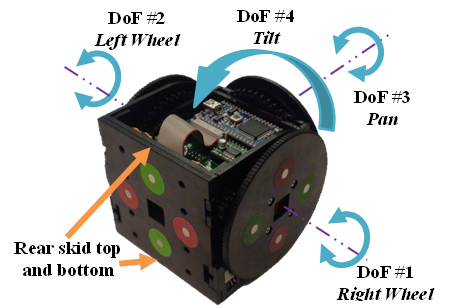
\includegraphics[height=1.2in]{images/smores_robot.png}
%   \{SMORES robot \TODO{Could this be combined with figure 1?  Use it
%   as the single module}}
%   \label{fig:SmoresRobot}
% \end{figure}

A design interface was implemented to aid users in building complex configurations and behaviors from a set of basic configurations and associated behaviors,
and then verifying their correct execution. We separated the program into two main parts: a configuration builder and a behavior builder.
%\subsection{Configuration Builder}
Given a set of basic configurations (which could be just single modules), the configuration builder allows users to combine basic configurations by choosing connection node on each configuration, as demonstrated in Figure~\ref{fig:smores_conf}. In addition, the configuration builder will warn users when the composed configuration is not valid without the usage of a physical simulator, e.g. Gazebo
\cite{koenig2004design}.

%\subsection{Behavior Builder}
Given a composed configuration, the behavior builder aids users in designing behaviors for the composed configuration by arranging a set of basic behaviors in parallel or in series. Figure~\ref{fig:smores_conf} illustrates a new behavior is composed by putting four basic behaviors in parallel. Similar to the configuration builder, the behavior builder will also warn users if there are self-collisions in the configuration during the execution of composed behaviors without simulations in a physical engine.

\begin{figure}
\begin{center}
    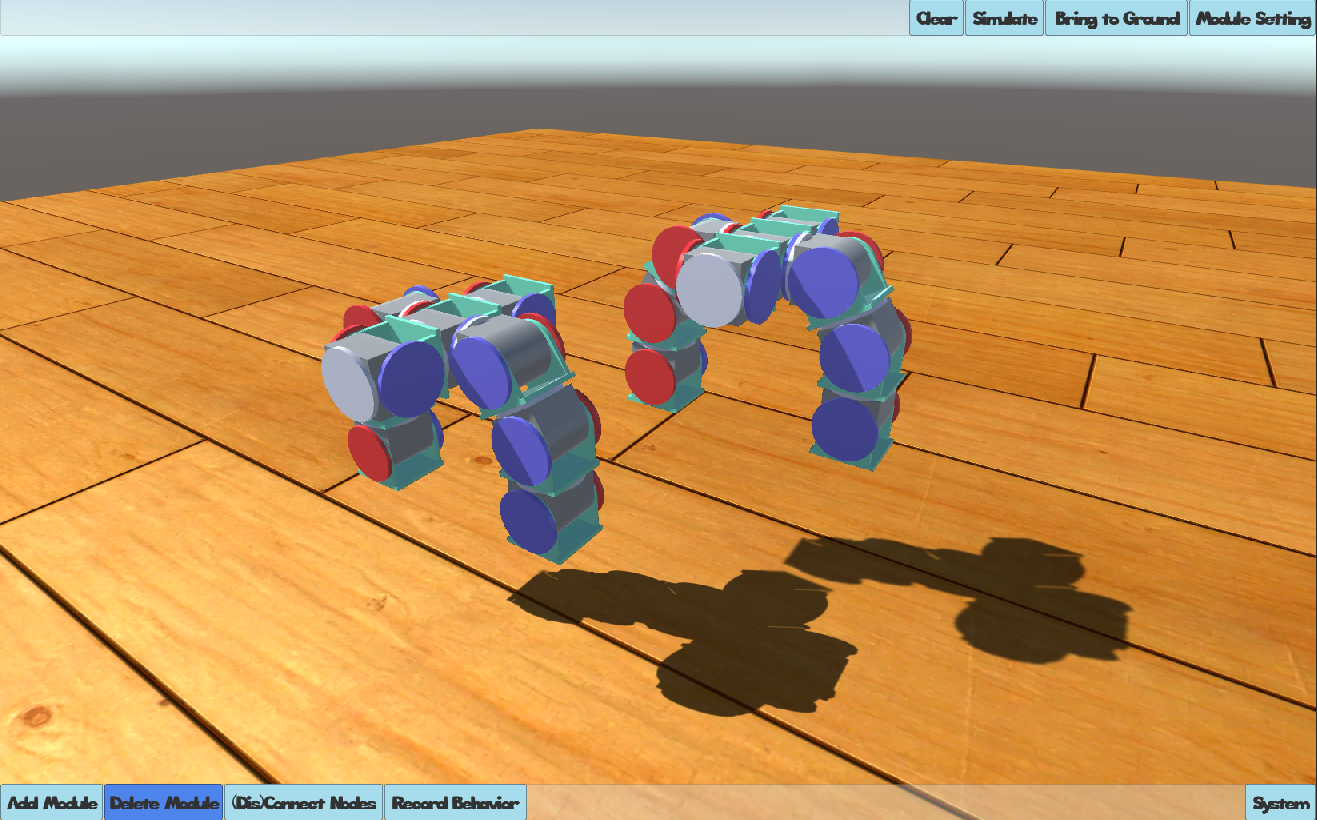
\includegraphics[height=1.1in]{images/library/unity/config_designer.png}
    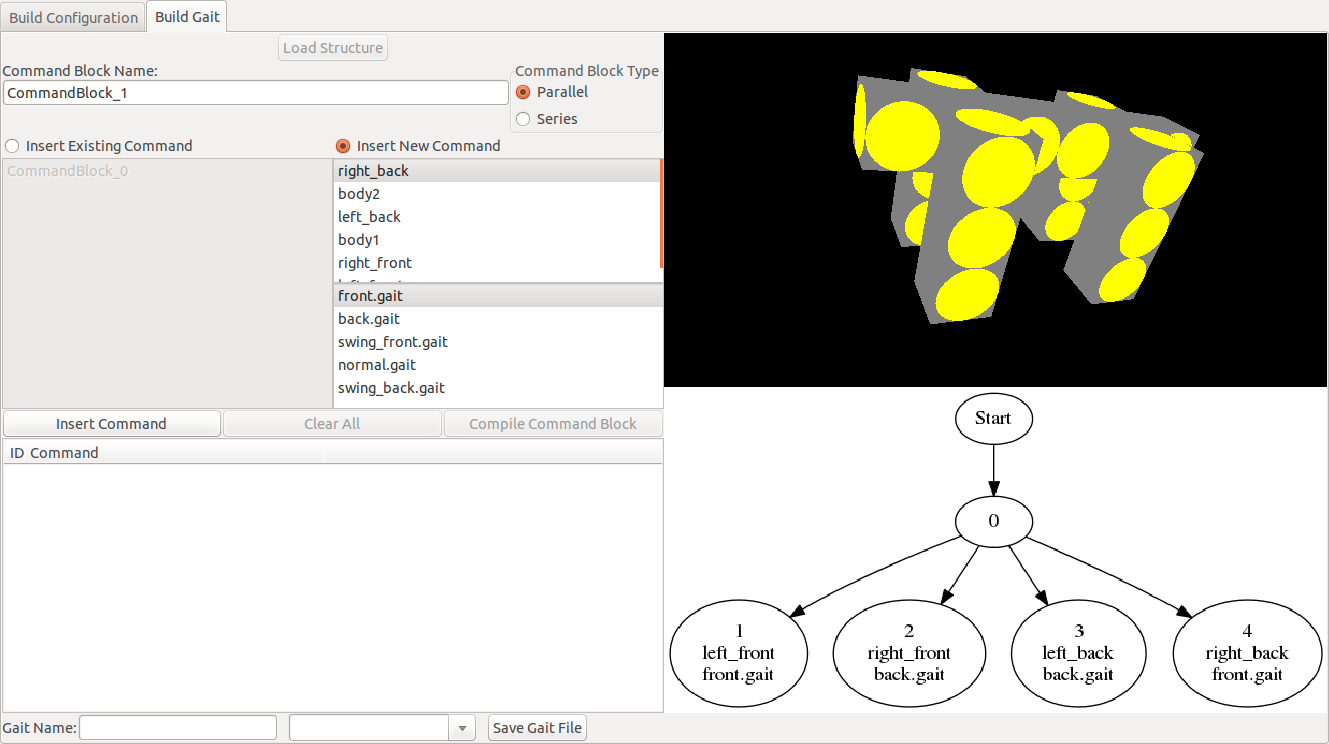
\includegraphics[height=1.1in]{images/gait_window.png}
    \caption{GUIs for configuration builder (left) and behavior builder (right)}
    \label{fig:smores_conf}
\end{center}
\end{figure}

% \begin{figure}
% \begin{center}
%         \begin{subfigure}[b]{0.49\columnwidth}
%                 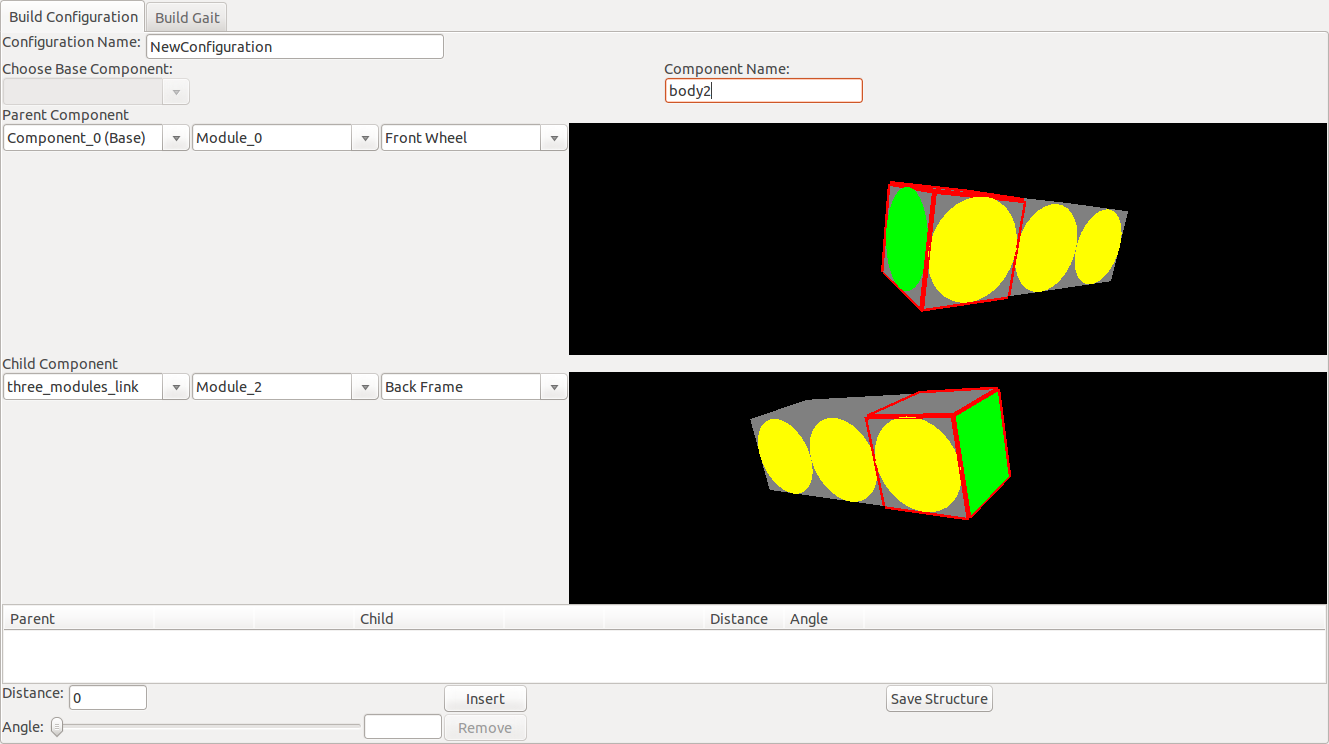
\includegraphics[width=\textwidth]{images/conf_window.png}
%                 \caption{GUI for configuration builder}
%                 \label{fig:gui_conf}
%         \end{subfigure}   
%         \begin{subfigure}[b]{0.49\columnwidth}
%                 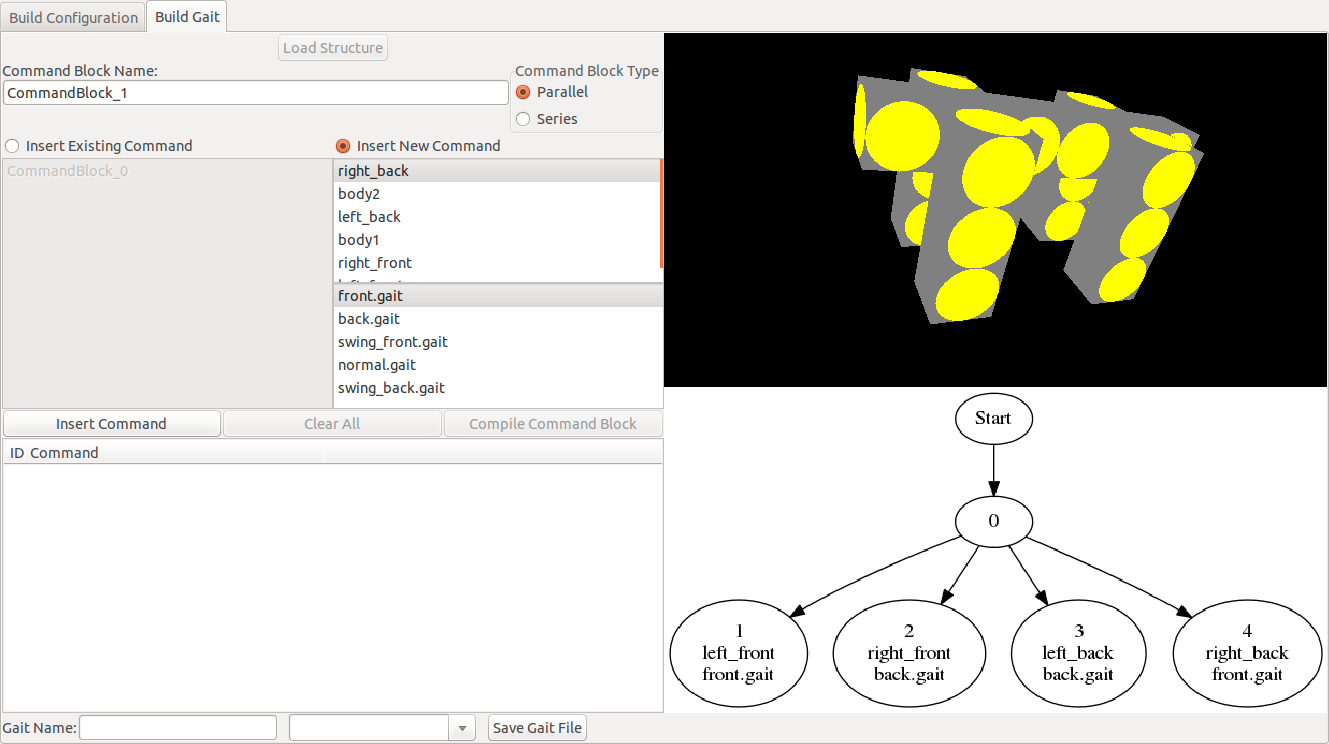
\includegraphics[width=\textwidth]{images/gait_window.png}
%                 \caption{GUI for behavior builder}
%                 \label{fig:gui_gait}
%         \end{subfigure}
% \end{center}
% \caption{The program to design and verify configurations and behaviors}
% \label{fig:smores_conf}
% \end{figure}
%
\section{Examples and User Perspective}
\label{sec:examples}
Our eventual intention is to develop a large library of configurations and associated
behaviors which are available to all users of our framework, analogous to the standard
libraries of major programming languages.  The compositional nature of our framework
will allow users to rely heavily on the library when approaching new tasks, allowing
them to create sophisticated robots very quickly.

As a first step toward a standard library, we present a small library of configurations
in Figure~\ref{fig:library}.
Configurations in the library are organized by \textit{order}, defined recursively
as follows: a single module is an order-zero configuration, and the order of all
other configurations is one greater than the largest order of the sub-configurations
from which it is composed. Each configuration has an associated set of behaviors,
which the user can compose to accomplish tasks.  New behaviors for higher-order configuration can be created by composing the behaviors of its component sub-configurations.

For the library to be most effective, the set of configurations and behaviors available
 at each level (and especially at the lowest levels) should provide a rich set of
 functionalities without presenting the user with an overwhelming number of options. 
 Considering the small library in Figure~\ref{fig:library},
 it is interested to note that a diverse set of second- and third-order configurations can
be constructed from only one zero- and one first-order configuration. Developing metrics to
evaluate the quality of such a library is an interesting opportunity for future work. 
%
% \begin{table*}
%      \begin{center}
%         \begin{tabular}{c c}
%          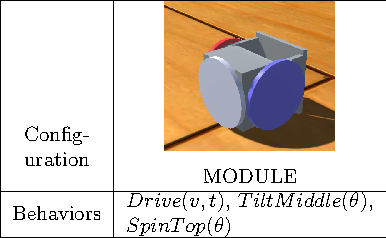
\includegraphics[scale=0.8]{images/library/tier0.pdf} &
%          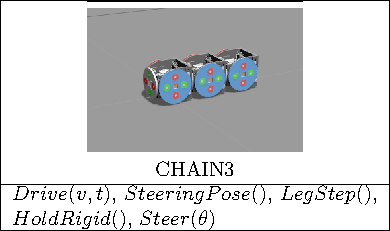
\includegraphics[scale=0.8]{images/library/tier1.pdf} \\
%          \textbf{Order-0 (single module)} & \textbf{Order-1}
%         \end{tabular}
%          \caption{Order-0 and Order-1 configurations}
%          \label{Order-1-configurations}
%      \end{center}
% \end{table*}
% \begin{table*}
%     \begin{center}
%         \begin{tabular}{c c}
%         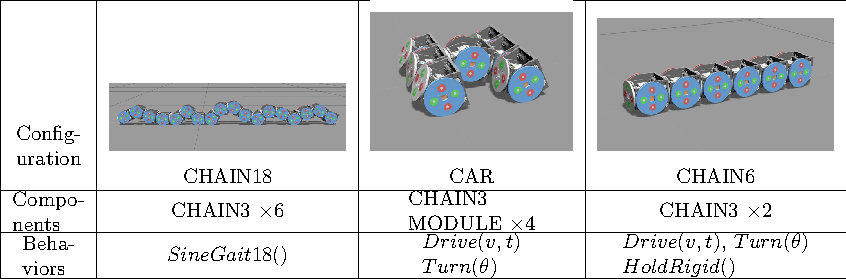
\includegraphics[scale=0.8]{images/library/tier2.pdf} &
%         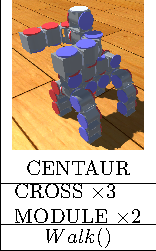
\includegraphics[scale=0.9]{images/library/tier3.pdf} \\
%         \textbf{Order-2} & \textbf{Order-3}
%         \end{tabular}
%         \caption{Order-2 and Order-3 configurations}
%         \label{Order-2-configurations}
%     \end{center}
% \end{table*}

\begin{figure}
  \begin{center}
    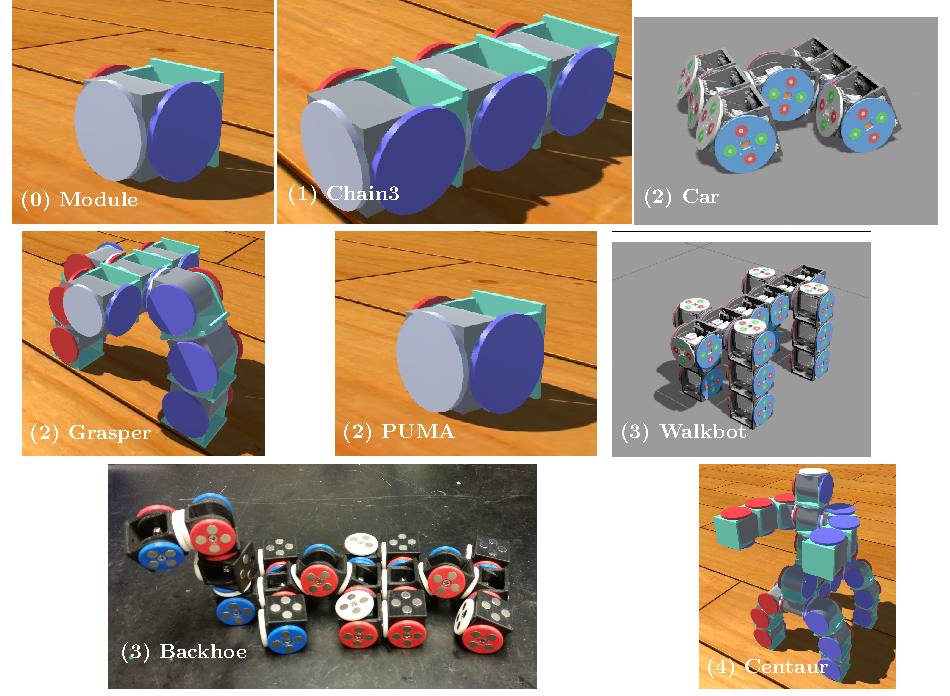
\includegraphics[width=\textwidth]{images/library/bigGrid.pdf}
    \caption{Library of designs, listed by order. 
    \textbf{Order 0:} Module. \textbf{Order 1:} Chain3=3x Module.
    \textbf{Order 2:} Car = Chain3 + 4x Module, Grasper = 3x Chain3, PUMA= Chain3 + Module.
    \textbf{Order 3:} Walkbot = 2x Grasper, Backhoe = 2x Car + PUMA.
    \textbf{Order 4:} Centaur = Walkbot + Grasper + 2x Module.}
    \label{fig:library}
  \end{center}
\end{figure}


% \begin{table*}
%     \begin{center}
%         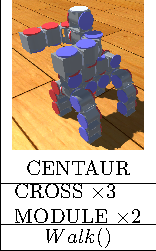
\includegraphics[scale=1]{images/library/tier3.pdf}
%         \caption{Order-3 configuration}
%         \label{Order-3-configurations}
%     \end{center}
% \end{table*}

%\subsection{The User Perspective}
Figure~\ref{fig:design} demonstrates the design flow when a user is designing a configuration an its behaviors. We present the start-to-end user perspective in designing a complicated configuration called Centaur. Consider the
order-1 `Chain3'' configuration. We can form a ``CROSS'' configuration. With two ``CROSS'' configuration, we can form a body, as demonstrated in Figure~\ref{fig:walkbot1}. With three more configurations attaching to the top of the body configuration with certain angle offset, we can build a complex configuration, Centaur, with four legs, as shown in Figure~\ref{fig:walkbot2}. Notice that by connecting multiple  basic configurations together, we can design a complex configuration more easily than creating with individual modules.

\begin{figure}
\begin{center}
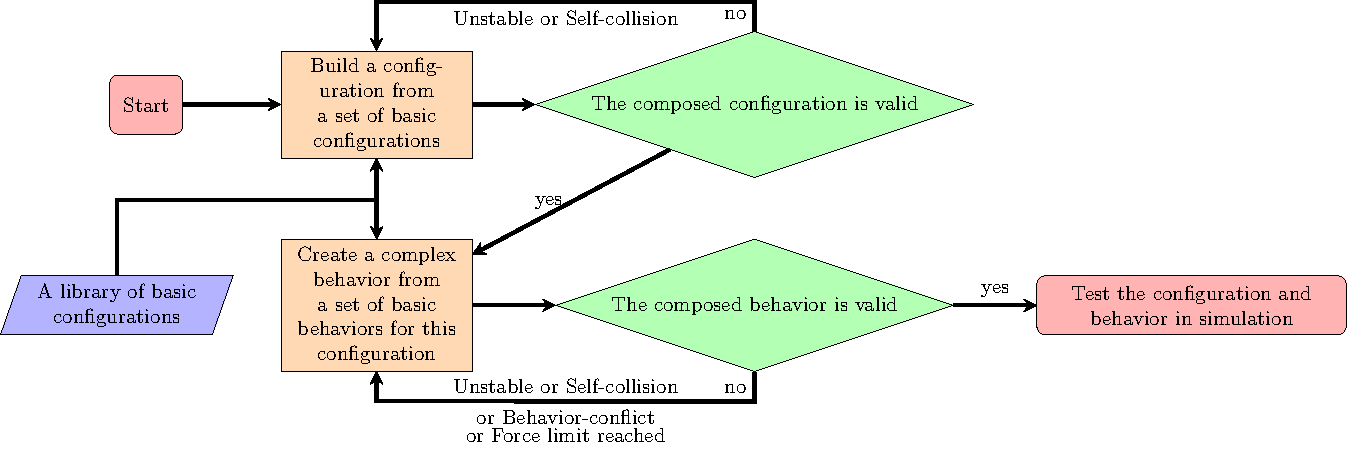
\includegraphics[width=\columnwidth]{images/tikz/design_diagram_hori.pdf}
\caption{The design flow}
\label{fig:design}
\end{center}
\end{figure}

\begin{figure}
\begin{center}
        \begin{subfigure}[b]{0.3\columnwidth}
                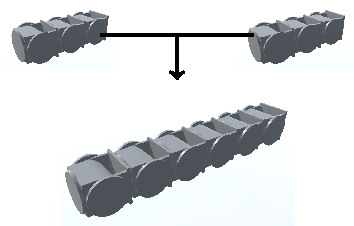
\includegraphics[width=\textwidth]{images/tikz/walkbot.pdf}
                \caption{Two identical configurations form a body}
                \label{fig:walkbot1}
        \end{subfigure}
        ~
        \begin{subfigure}[b]{0.65\columnwidth}
                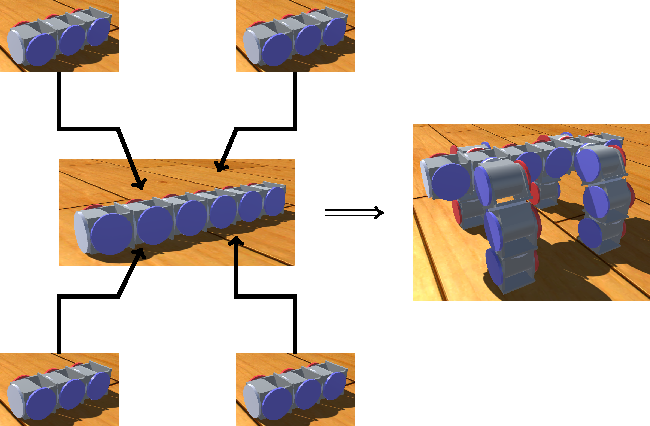
\includegraphics[width=\textwidth]{images/tikz/walkbot2.pdf}
                \caption{The body and other configurations form a Centaur}
                \label{fig:walkbot2}
        \end{subfigure}
\end{center}
\caption{Building a Centaur with a set of configurations}
\label{fig:walkbot}
\end{figure}

%\subsection{Scale-up through composition}
% Our framework allows users to quickly create and program large configurations. The
% first-order CHAIN3 configuration (Table~\ref{Order-1-configurations}) can use a \(sineGait\)
% behavior to locomote like a snake. Defining \(sineGait\)  as the series composition
% of two half-waves will allow us to re-use the gait with larger snakes:
% \begin{displaymath}
% sineGait = Sc(~halfSine1,~halfSine2~)
% \end{displaymath}
% Arbitrarily long snake configurations can be created
% by composing CHAIN3 configurations end-to-end; Table~\ref{Order-2-configurations} shows one with 18 modules.
% A gait for an arbitrarily long snake is created by composing sine wave
% gaits for each component in parallel, but with alternating phase:
% \begin{align*}
% nSnakeSineGait = ~~~~~~~~~~~~~~~~~~~~~~~~~~~~~~~~~~~~~~~~~~\\
% Pc \left(~Sc\begin{pmatrix} halfSine1 \\ halfSine2 \end{pmatrix},
% ~Sc\begin{pmatrix} halfSine2 \\ halfSine1 \end{pmatrix},\ldots ~\right)
% \end{align*}

% \subsection{Verification}
% The need for verification becomes more important as design complexity increases. Consider a four-legged Walkbot example. If the user sets two of the connections with different angle offset, the composed Walkbot configuration will have two legs pointing in the opposite direction of the other two legs, as shown in Figure~\ref{fig:designer_unstable}. Since the projection of the configuration's center of mass now falls out of the supporting base, the program will warn the user that the configuration is not gravitationally stable. As shown in Figure~\ref{fig:gazebo_unstable2}, in simulation the configuration quickly fell to the ground due to the instability as warned by the program. 
% 
% Verification of behavior design can also aid the user to create valid and safe robot behaviors. When designing the walking behavior for the Walkbot, if the user commands the front and rear leg at the same side of the robot to swing toward each other at the same time, the program will warn the user that there will be collision between some modules in this behavior, as shown in Figure~\ref{fig:gait_collision}. The photo shown in Figure~\ref{fig:gait_collision2} demonstrates the moment of collision during simulation.
% 
% Despite the design of the modular robot system, modules all have limits on maximum force that is available to maintain connections with other modules and to drive each joint to desired positions. Thus, it is crucial to notify the user if there is no sufficient force from module's hardware to execute a behavior while maintaining all modules connections. 
% As shown in Figure~\ref{fig:break_joint1}, the program detected an undesired disconnection when the user tried to lift a long cantilever arm. Figure~\ref{fig:break_joint1} demonstrates the disconnection in simulation.
%  
% \begin{figure}
% \begin{center}
%         \begin{subfigure}[b]{0.48\columnwidth}
%                 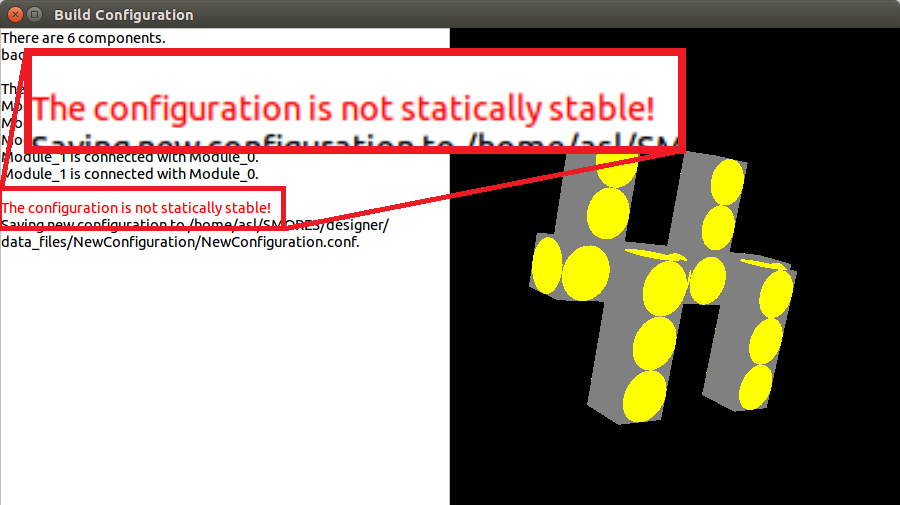
\includegraphics[width=\textwidth]{images/designer_unstable.png}
%                 \caption{}
%                 \label{fig:designer_unstable}
%            \end{subfigure}
%         \begin{subfigure}[b]{0.48\columnwidth}
%                 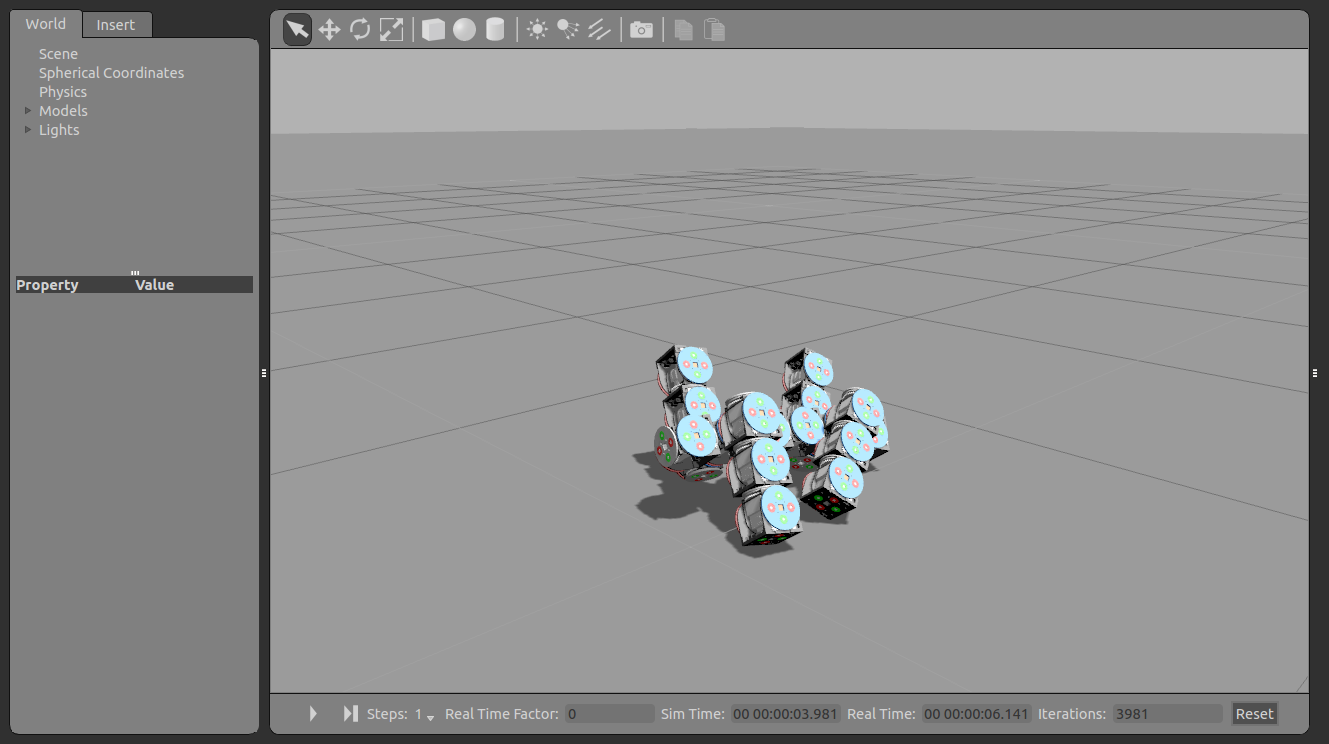
\includegraphics[width=\textwidth]{images/gazebo_unstable2.png}
%                 \caption{}
%                 \label{fig:gazebo_unstable2}
%         \end{subfigure}
% \end{center}
% \caption{(a) The program warns the composed configuration is not gravitationally stable; (b) The robot fell to ground plane due to instability in simulation}
% \label{fig:unstable}
% \end{figure}
% 
% \begin{figure}
% \begin{center}
%         \begin{subfigure}[b]{0.48\columnwidth}
%                 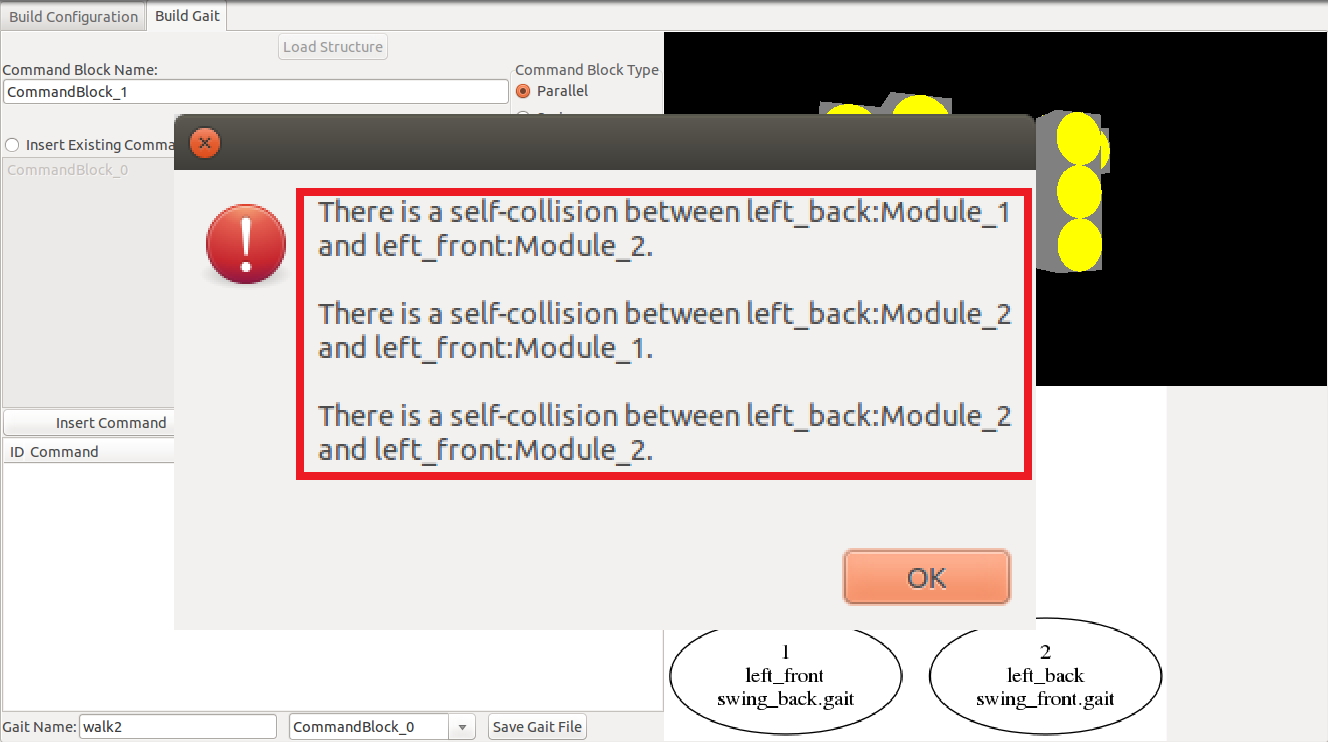
\includegraphics[width=\textwidth]{images/designer_gait_collision.png}
%                 \caption{}
%                 \label{fig:gait_collision}
%            \end{subfigure}
%         \begin{subfigure}[b]{0.48\columnwidth}
%                 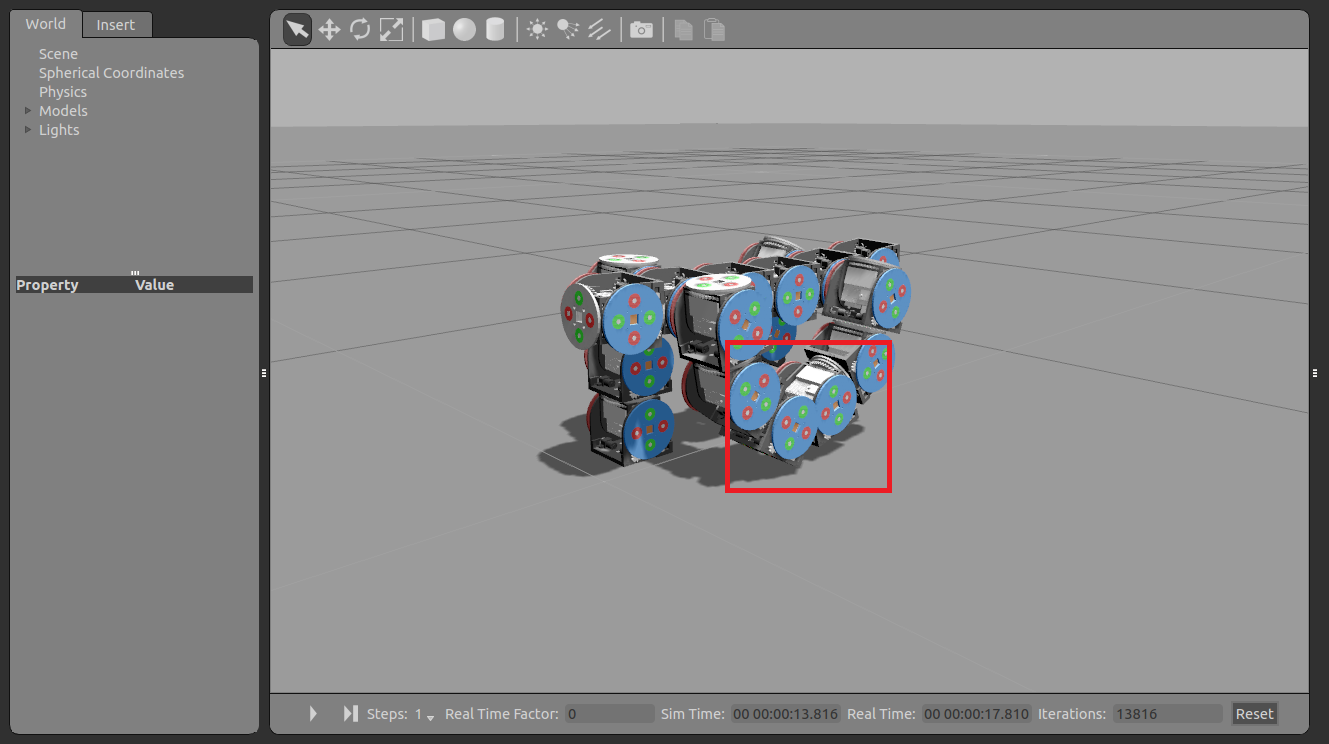
\includegraphics[width=\textwidth]{images/gazebo_gait_collision.png}
%                 \caption{}
%                 \label{fig:gait_collision2}
%         \end{subfigure}
% \end{center}
% \caption{(a) The program indicates there is collision during the behavior execution; (b) Two feet of  the robot collided during simulation}
% \label{fig:gait_unstable}
% \end{figure}
% 
% \begin{figure}
% \begin{center}
%         \begin{subfigure}[b]{0.48\columnwidth}
%                 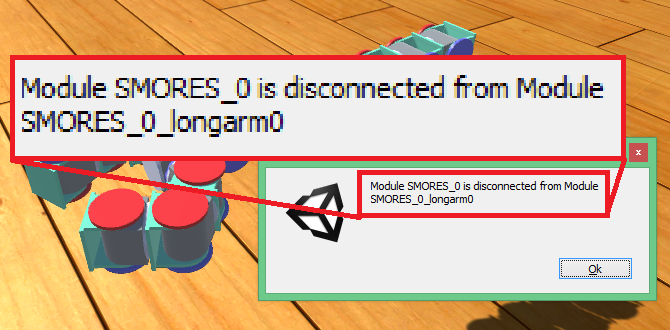
\includegraphics[width=\textwidth]{images/library/unity/breakJoint.png}
%                 \caption{}
%                 \label{fig:break_joint1}
%            \end{subfigure}
%         \begin{subfigure}[b]{0.48\columnwidth}
%                 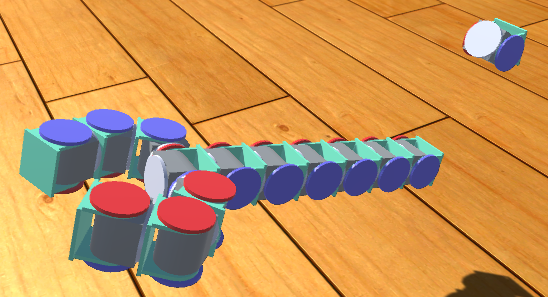
\includegraphics[width=\textwidth]{images/library/unity/breakJoint2.png}
%                 \caption{}
%                 \label{fig:break_joint2}
%         \end{subfigure}
% \end{center}
% \caption{(a) The program indicates there is undesired disconnection; (b) The configuration disconnected during simulation}
% \label{fig:break_joint}
% \end{figure}


\section{Results}
In the past, designing configurations and behaviors to address new tasks has required
time on the order of one to dozens of hours \cite{sastra2011using}.  To evaluate the rapid creation of solutions for robotic tasks using modular robot systems, we can look to the modular robot competitions held at large conferences IROS 2003, ICRA 2008, ICRA 2010, ICRA 2011 and ICRA 2012. In each case participants used modular robot systems to solve problems with little a priori knowledge of the task (except that the task would likely require remote operation/manipulation of objects).

In the case of IROS 2003, the task was to create a robot that could ``gamble'' by placing plastic tokens into a toy slot machine, pulling a lever and catching the chips as they popped out.  One team created a solution with PolyBot G1V4 system with 14 modules (14 DoF). Participants
had one day to create primitive configurations and behaviors (snake-like mobility, and arm like structures) and
 6 hours on the following day to solve the task. No teams completed the task, though
some came close. 
At ICRA 2008, participants created designs to address a mock disaster scenario
at a space station on Mars. Teams spent on average about 3 hours building configurations and
3 hours programming them to address the task \cite{sastra2011using}.  
  
Using our framework and library, a single person has created and programmed   configurations of similar complexity to those used at
the competitions (such as the Centaur or 18-module snake)
in under an hour,
or in a few minutes if the right primitives already exist in the library. Figure~\ref{fig:walk} shows a four-step walking behavior for the Centaur. It would
not be fair to compare these times to the competition times directly, since they do not include any
hardware tests or hardware debugging. However, we think we can safely say that
our framework is an improvement over past design practices.
%
% \begin{figure}
% \begin{center}
%         \begin{subfigure}[b]{0.23\columnwidth}
%                 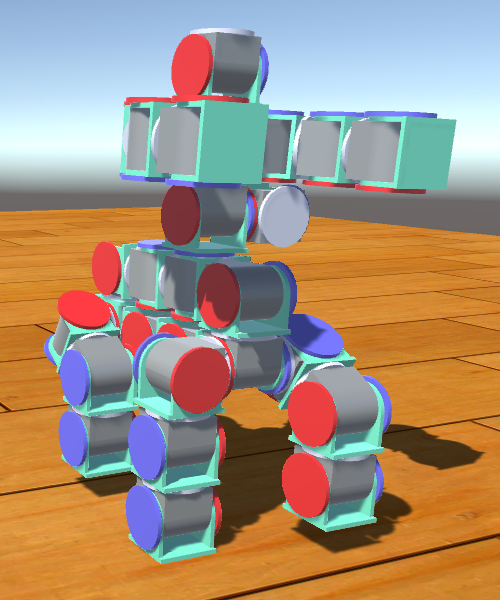
\includegraphics[width=\textwidth]{images/library/unity/step1.png}
%                 \caption{}
%                 \label{fig:step1}
%            \end{subfigure}
%         \begin{subfigure}[b]{0.23\columnwidth}
%                 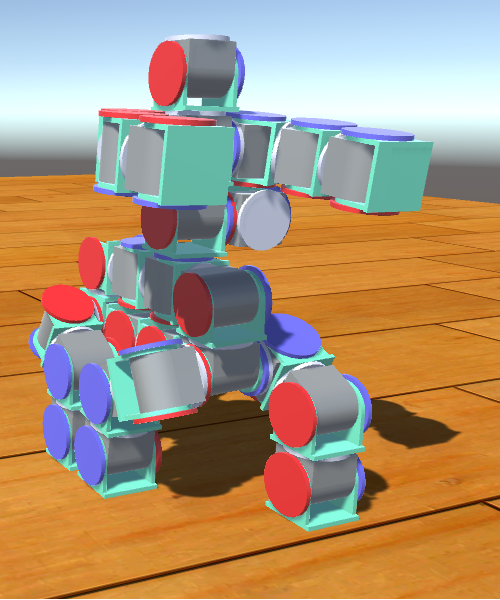
\includegraphics[width=\textwidth]{images/library/unity/step2.png}
%                 \caption{}
%                 \label{fig:step2}
%         \end{subfigure}
%         \begin{subfigure}[b]{0.23\columnwidth}
%                 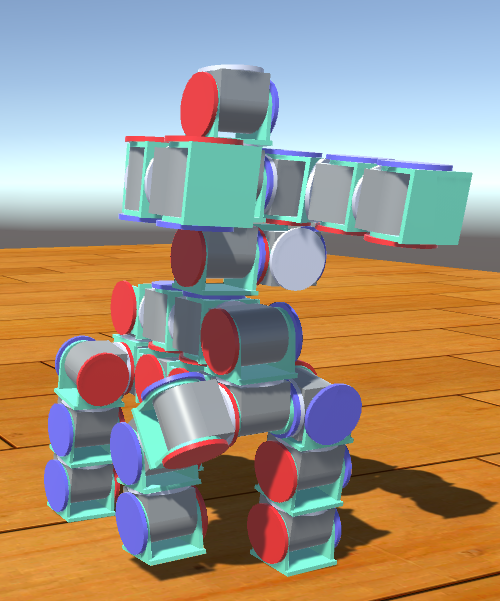
\includegraphics[width=\textwidth]{images/library/unity/step3.png}
%                 \caption{}
%                 \label{fig:step3}
%            \end{subfigure}
%         \begin{subfigure}[b]{0.23\columnwidth}
%                 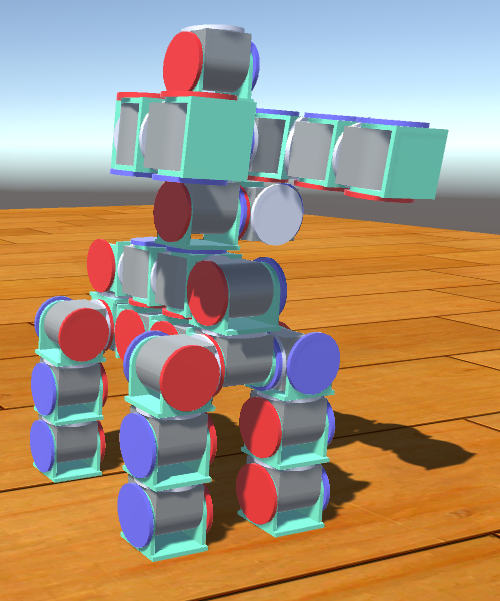
\includegraphics[width=\textwidth]{images/library/unity/step4.png}
%                 \caption{}
%                 \label{fig:step4}
%         \end{subfigure}
% \end{center}
% \caption{A four-step walking behavior}
% \label{fig:walk}
% \end{figure}
\begin{figure}
\begin{center}
                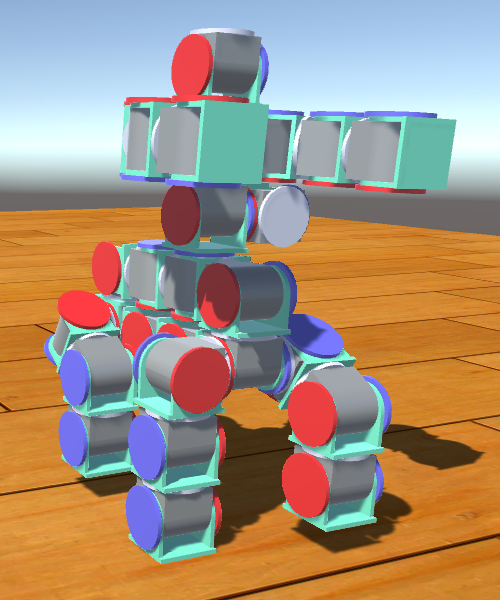
\includegraphics[width=0.23\textwidth]{images/library/unity/step1.png}
                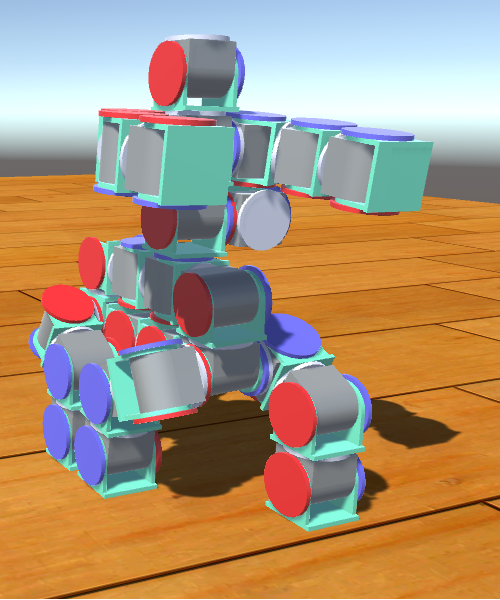
\includegraphics[width=0.23\textwidth]{images/library/unity/step2.png}
                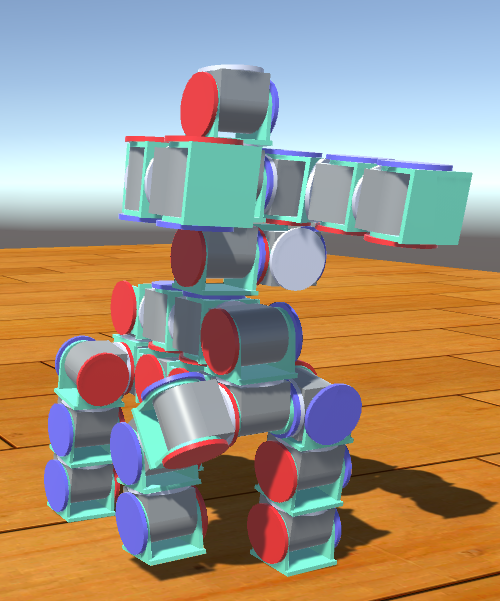
\includegraphics[width=0.23\textwidth]{images/library/unity/step3.png}
                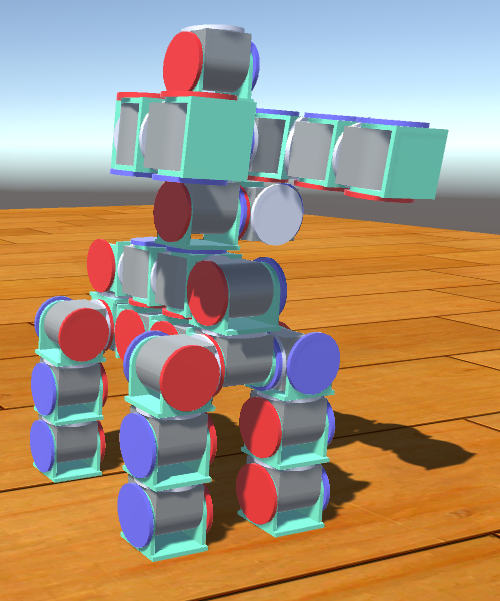
\includegraphics[width=0.23\textwidth]{images/library/unity/step4.png}
\end{center}
\caption{A four-step walking behavior}
\label{fig:walk}
\end{figure}


\section{Conclusions}
In this paper, we presented a design framework that facilitates the rapid creation
of configurations and behaviors for modular robots.
Complex configurations  are hierarchically constructed from basic
subcomponents.
We presented a novel motion description language, which allows existing behaviors
to be combined in series and parallel  to create more complex  behaviors.
The framework verifies  configurations and behaviors as they are being created, allowing
early detection of  design flaws, specifically self-collision and gravitational instability. After
verification, designs can be evaluated in a physical simulator before testing on
hardware.

\section{Future}
Future work will include expansion of the features of our framework.  We will add verification tools to check for behavior conflict (when two behaviors composed in parallel command the same DoF), and check for behaviors that would exceed the actuator and connector force limits of the modules.  We will also work to include configurations with cycles.
Another area of future work is developing a standard library of configurations and
behaviors for the SMORES robot.  We will also investigate metrics to evaluate the quality of such a library.
Perhaps most importantly, we will test and evaluate the designs and behaviors with actual hardware modules.
Currently, each behavior is associated with exactly one configuration. In many cases, a given behavior could be executed by several different configurations (if it were correctly mapped onto a subset of their modules). In the future, we will apply an embedding detection algorithm (see \cite{mantzouratos2014embeddability}) to map behaviors into any configuration capable of executing them.

%%%%%%%%%%%%%%%%%%%%%%%%% referenc.tex %%%%%%%%%%%%%%%%%%%%%%%%%%%%%%
% sample references
% %
% Use this file as a template for your own input.
%
%%%%%%%%%%%%%%%%%%%%%%%% Springer-Verlag %%%%%%%%%%%%%%%%%%%%%%%%%%
%
% BibTeX users please use
% \bibliographystyle{}
% \bibliography{}
%
\biblstarthook{References may be \textit{cited} in the text either by number (preferred) or by author/year.\footnote{Make sure that all references from the list are cited in the text. Those not cited should be moved to a separate \textit{Further Reading} section or chapter.} The reference list should ideally be \textit{sorted} in alphabetical order -- even if reference numbers are used for the their citation in the text. If there are several works by the same author, the following order should be used: 
\begin{enumerate}
\item all works by the author alone, ordered chronologically by year of publication
\item all works by the author with a coauthor, ordered alphabetically by coauthor
\item all works by the author with several coauthors, ordered chronologically by year of publication.
\end{enumerate}
The \textit{styling} of references\footnote{Always use the standard abbreviation of a journal's name according to the ISSN \textit{List of Title Word Abbreviations}, see \url{http://www.issn.org/en/node/344}} depends on the subject of your book:
\begin{itemize}
\item The \textit{two} recommended styles for references in books on \textit{mathematical, physical, statistical and computer sciences} are depicted in ~\cite{science-contrib, science-online, science-mono, science-journal, science-DOI} and ~\cite{phys-online, phys-mono, phys-journal, phys-DOI, phys-contrib}.
\item Examples of the most commonly used reference style in books on \textit{Psychology, Social Sciences} are~\cite{psysoc-mono, psysoc-online,psysoc-journal, psysoc-contrib, psysoc-DOI}.
\item Examples for references in books on \textit{Humanities, Linguistics, Philosophy} are~\cite{humlinphil-journal, humlinphil-contrib, humlinphil-mono, humlinphil-online, humlinphil-DOI}.
\item Examples of the basic Springer style used in publications on a wide range of subjects such as \textit{Computer Science, Economics, Engineering, Geosciences, Life Sciences, Medicine, Biomedicine} are ~\cite{basic-contrib, basic-online, basic-journal, basic-DOI, basic-mono}. 
\end{itemize}
}

\begin{thebibliography}{99.}%
% and use \bibitem to create references.
%
% Use the following syntax and markup for your references if 
% the subject of your book is from the field 
% "Mathematics, Physics, Statistics, Computer Science"
%
% Contribution 
\bibitem{science-contrib} Broy, M.: Software engineering --- from auxiliary to key technologies. In: Broy, M., Dener, E. (eds.) Software Pioneers, pp. 10-13. Springer, Heidelberg (2002)
%
% Online Document
\bibitem{science-online} Dod, J.: Effective substances. In: The Dictionary of Substances and Their Effects. Royal Society of Chemistry (1999) Available via DIALOG. \\
\url{http://www.rsc.org/dose/title of subordinate document. Cited 15 Jan 1999}
%
% Monograph
\bibitem{science-mono} Geddes, K.O., Czapor, S.R., Labahn, G.: Algorithms for Computer Algebra. Kluwer, Boston (1992) 
%
% Journal article
\bibitem{science-journal} Hamburger, C.: Quasimonotonicity, regularity and duality for nonlinear systems of partial differential equations. Ann. Mat. Pura. Appl. \textbf{169}, 321--354 (1995)
%
% Journal article by DOI
\bibitem{science-DOI} Slifka, M.K., Whitton, J.L.: Clinical implications of dysregulated cytokine production. J. Mol. Med. (2000) doi: 10.1007/s001090000086 
%
\bigskip

% Use the following (APS) syntax and markup for your references if 
% the subject of your book is from the field 
% "Mathematics, Physics, Statistics, Computer Science"
%
% Online Document
\bibitem{phys-online} J. Dod, in \textit{The Dictionary of Substances and Their Effects}, Royal Society of Chemistry. (Available via DIALOG, 1999), 
\url{http://www.rsc.org/dose/title of subordinate document. Cited 15 Jan 1999}
%
% Monograph
\bibitem{phys-mono} H. Ibach, H. L\"uth, \textit{Solid-State Physics}, 2nd edn. (Springer, New York, 1996), pp. 45-56 
%
% Journal article
\bibitem{phys-journal} S. Preuss, A. Demchuk Jr., M. Stuke, Appl. Phys. A \textbf{61}
%
% Journal article by DOI
\bibitem{phys-DOI} M.K. Slifka, J.L. Whitton, J. Mol. Med., doi: 10.1007/s001090000086
%
% Contribution 
\bibitem{phys-contrib} S.E. Smith, in \textit{Neuromuscular Junction}, ed. by E. Zaimis. Handbook of Experimental Pharmacology, vol 42 (Springer, Heidelberg, 1976), p. 593
%
\bigskip
%
% Use the following syntax and markup for your references if 
% the subject of your book is from the field 
% "Psychology, Social Sciences"
%
%
% Monograph
\bibitem{psysoc-mono} Calfee, R.~C., \& Valencia, R.~R. (1991). \textit{APA guide to preparing manuscripts for journal publication.} Washington, DC: American Psychological Association.
%
% Online Document
\bibitem{psysoc-online} Dod, J. (1999). Effective substances. In: The dictionary of substances and their effects. Royal Society of Chemistry. Available via DIALOG. \\
\url{http://www.rsc.org/dose/Effective substances.} Cited 15 Jan 1999.
%
% Journal article
\bibitem{psysoc-journal} Harris, M., Karper, E., Stacks, G., Hoffman, D., DeNiro, R., Cruz, P., et al. (2001). Writing labs and the Hollywood connection. \textit{J Film} Writing, 44(3), 213--245.
%
% Contribution 
\bibitem{psysoc-contrib} O'Neil, J.~M., \& Egan, J. (1992). Men's and women's gender role journeys: Metaphor for healing, transition, and transformation. In B.~R. Wainrig (Ed.), \textit{Gender issues across the life cycle} (pp. 107--123). New York: Springer.
%
% Journal article by DOI
\bibitem{psysoc-DOI}Kreger, M., Brindis, C.D., Manuel, D.M., Sassoubre, L. (2007). Lessons learned in systems change initiatives: benchmarks and indicators. \textit{American Journal of Community Psychology}, doi: 10.1007/s10464-007-9108-14.
%
%
% Use the following syntax and markup for your references if 
% the subject of your book is from the field 
% "Humanities, Linguistics, Philosophy"
%
\bigskip
%
% Journal article
\bibitem{humlinphil-journal} Alber John, Daniel C. O'Connell, and Sabine Kowal. 2002. Personal perspective in TV interviews. \textit{Pragmatics} 12:257--271
%
% Contribution 
\bibitem{humlinphil-contrib} Cameron, Deborah. 1997. Theoretical debates in feminist linguistics: Questions of sex and gender. In \textit{Gender and discourse}, ed. Ruth Wodak, 99--119. London: Sage Publications.
%
% Monograph
\bibitem{humlinphil-mono} Cameron, Deborah. 1985. \textit{Feminism and linguistic theory.} New York: St. Martin's Press.
%
% Online Document
\bibitem{humlinphil-online} Dod, Jake. 1999. Effective substances. In: The dictionary of substances and their effects. Royal Society of Chemistry. Available via DIALOG. \\
http://www.rsc.org/dose/title of subordinate document. Cited 15 Jan 1999
%
% Journal article by DOI
\bibitem{humlinphil-DOI} Suleiman, Camelia, Daniel C. O�Connell, and Sabine Kowal. 2002. `If you and I, if we, in this later day, lose that sacred fire...�': Perspective in political interviews. \textit{Journal of Psycholinguistic Research}. doi: 10.1023/A:1015592129296.
%
%
%
\bigskip
%
%
% Use the following syntax and markup for your references if 
% the subject of your book is from the field 
% "Computer Science, Economics, Engineering, Geosciences, Life Sciences"
%
%
% Contribution 
\bibitem{basic-contrib} Brown B, Aaron M (2001) The politics of nature. In: Smith J (ed) The rise of modern genomics, 3rd edn. Wiley, New York 
%
% Online Document
\bibitem{basic-online} Dod J (1999) Effective Substances. In: The dictionary of substances and their effects. Royal Society of Chemistry. Available via DIALOG. \\
\url{http://www.rsc.org/dose/title of subordinate document. Cited 15 Jan 1999}
%
% Journal article by DOI
\bibitem{basic-DOI} Slifka MK, Whitton JL (2000) Clinical implications of dysregulated cytokine production. J Mol Med, doi: 10.1007/s001090000086
%
% Journal article
\bibitem{basic-journal} Smith J, Jones M Jr, Houghton L et al (1999) Future of health insurance. N Engl J Med 965:325--329
%
% Monograph
\bibitem{basic-mono} South J, Blass B (2001) The future of modern genomics. Blackwell, London 
%
\end{thebibliography}

%\bibliographystyle{plainnat}
\bibliographystyle{spmpsci}
\bibliography{references}
\end{document}

























